\documentclass[conference]{IEEEtran}

\usepackage{graphicx}
\usepackage{amsmath,amssymb}
\usepackage{cite}
\usepackage{booktabs}
\usepackage{multirow}
\usepackage{tabularx}
\usepackage{url}
\usepackage{xurl}
\usepackage{pgfplots}
\usepackage[hidelinks]{hyperref}
\usepackage[caption=false,font=footnotesize]{subfig}
\pgfplotsset{compat=1.18}

\graphicspath{{./}{./figures/}{./tables/}}

% Result macros from verified model runs.
\newcommand{\aucLR}{0.822}
\newcommand{\aucNB}{0.698}
\newcommand{\aucSVM}{0.836}
\newcommand{\aucCNN}{0.858}
\newcommand{\aucEnsemble}{0.929}

\title{Detection and Risk Assessment of Unsafe Hanging Travel in Public Transport Using Machine Learning}

\author{\IEEEauthorblockN{Tazkia Malik, Sadek Hossain Asif, Tanzila Khan, Taif Ahmed Turjo, Amio Rashid, Mahmud Hasan Walid}
\IEEEauthorblockA{Department of Computer Science and Engineering\\
University of Dhaka\\
Dhaka, Bangladesh}}

\begin{document}
\maketitle

\begin{abstract}
Unsafe door-hanging and overcrowded travel are persistent safety risks in Dhaka's public transport system, particularly in buses and legunas operating under high passenger demand. Existing intelligent transportation research has addressed vehicle detection, passenger counting, and general crowd analysis, but localized automated detection of unsafe hanging travel remains limited. This paper presents an image-based machine-learning framework for classifying public transport scenes into safe/normal and unsafe/risky conditions. A custom bus and leguna image dataset is prepared through cleaning, annotation, preprocessing, and augmentation. For classical machine-learning baselines, Histogram of Oriented Gradients (HOG) descriptors are used with Logistic Regression, Gaussian Naive Bayes, and a Support Vector Machine (SVM) with a radial basis function kernel. Deep models including a CNN trained from scratch, ResNet18, EfficientNet-B0, ResNet50, ConvNeXt-Tiny, and an ensemble are also evaluated to compare learned visual features with handcrafted HOG representations. The models are assessed using accuracy, unsafe-class recall, confusion matrices, and AUC. The updated results show that automated visual screening of unsafe hanging travel is feasible on a modest localized dataset, with the ResNet50--ConvNeXt ensemble achieving the strongest balanced cross-validated performance and SVM remaining the strongest classical baseline by AUC.
\end{abstract}

\begin{IEEEkeywords}
Unsafe public transport, computer vision, image classification, Histogram of Oriented Gradients, support vector machine, convolutional neural network, intelligent transportation system.
\end{IEEEkeywords}

\section{Introduction}
Public transport in Dhaka carries a large share of daily urban mobility, but high passenger demand, limited vehicle capacity, and inconsistent enforcement often create unsafe conditions. A common visible hazard is door-hanging travel, where passengers ride from the doorway or exterior boundary of buses and legunas, increasing exposure to falls, collisions, and roadside obstacles.

Safety monitoring still depends heavily on traffic personnel, transport operators, or surveillance staff. Manual observation is difficult to scale across dense road networks, heterogeneous vehicle types, and continuously changing traffic scenes.

Computer vision is useful for this task because images can capture vehicle structure, passenger position, crowding, and doorway conditions. This paper proposes an image-based machine-learning system that classifies Dhaka public transport scenes into safe/normal negative samples and unsafe/risky positive samples.

The main contributions are as follows:
\begin{itemize}
    \item A localized safe/unsafe public transport image dataset containing Dhaka bus and leguna scenes.
    \item A complete machine-learning pipeline for unsafe hanging-travel detection.
    \item A comparison of HOG-based classical machine-learning models and deep convolutional models.
    \item An evaluation using standard classification metrics, including accuracy, unsafe-class recall, confusion matrices, AUC, and learning curves where applicable.
\end{itemize}

\section{Related Work}
Computer vision has become an important component of intelligent transportation systems. Surveyed applications include vehicle detection, pedestrian detection, anomaly detection, traffic monitoring, and automatic number-plate recognition \cite{dilek2023cvits}. These methods show that visual data can support automated interpretation of transportation scenes, although most work targets general traffic understanding rather than specific passenger-safety risks.

Passenger monitoring research commonly focuses on counting, occupancy estimation, boarding analysis, and crowd monitoring in buses or terminals \cite{hsu2020passenger}. Public transport safety studies identify overcrowding, weak enforcement, and unsafe passenger behavior as important risk factors in dense urban environments \cite{hossain2018bus}, while broader reviews show that crowd pressure and non-collision incidents remain persistent concerns when demand exceeds service capacity \cite{crowding2023review}.

Unsafe behavior and abnormal-activity detection are related to the present task because they aim to identify visual patterns that deviate from normal scenes. Recent surveys report that deep learning can be effective for abnormal behavior detection, but they also emphasize difficulties caused by limited labeled data, occlusion, scene variation, and domain transfer \cite{wastupranata2024abnormal}. Object-detection methods such as YOLO provide another foundation for transportation surveillance and boarding or alighting recognition \cite{redmon2016yolo}, \cite{yolo2024boarding}.

Automatic License Plate Recognition (ALPR) is relevant only as future context for identifying vehicles after unsafe behavior is detected. Existing ALPR studies address plate localization and recognition under real-world imaging constraints \cite{anagnostopoulos2008license}, \cite{silva2018license}, \cite{du2013automatic}, including Bengali license-plate recognition under low-resolution and blurred conditions \cite{afrin2023bengali}.

The key gap is that existing work rarely addresses unsafe door-hanging detection in Dhaka-like crowded public transport environments using localized datasets under real-world challenges such as occlusion, motion blur, lighting variation, crowding, and non-standard vehicle structures. Prior systems often estimate occupancy, count passengers, or recognize boarding events, but they do not directly model hanging passengers as a safety-critical positive class under local bus and leguna conditions.

\section{Dataset}
\subsection{Data Collection}
The dataset contains images of buses and legunas captured under real-world public transport conditions in Dhaka. The samples cover safe/normal and unsafe/risky cases with variation in vehicle type, passenger density, camera angle, lighting, and scene clutter. In the updated result set, labels are taken from image annotations: an unsafe box indicates unsafe hanging travel, while license-plate boxes are ignored for the classification label. After collection, cleaning, relabeling from annotations, and standardization, the model-development set contains 385 images, with 287 safe samples and 98 unsafe samples. Figure~\ref{fig:eda} summarizes the updated class distribution and split composition.

\begin{figure}[!t]
    \centering
    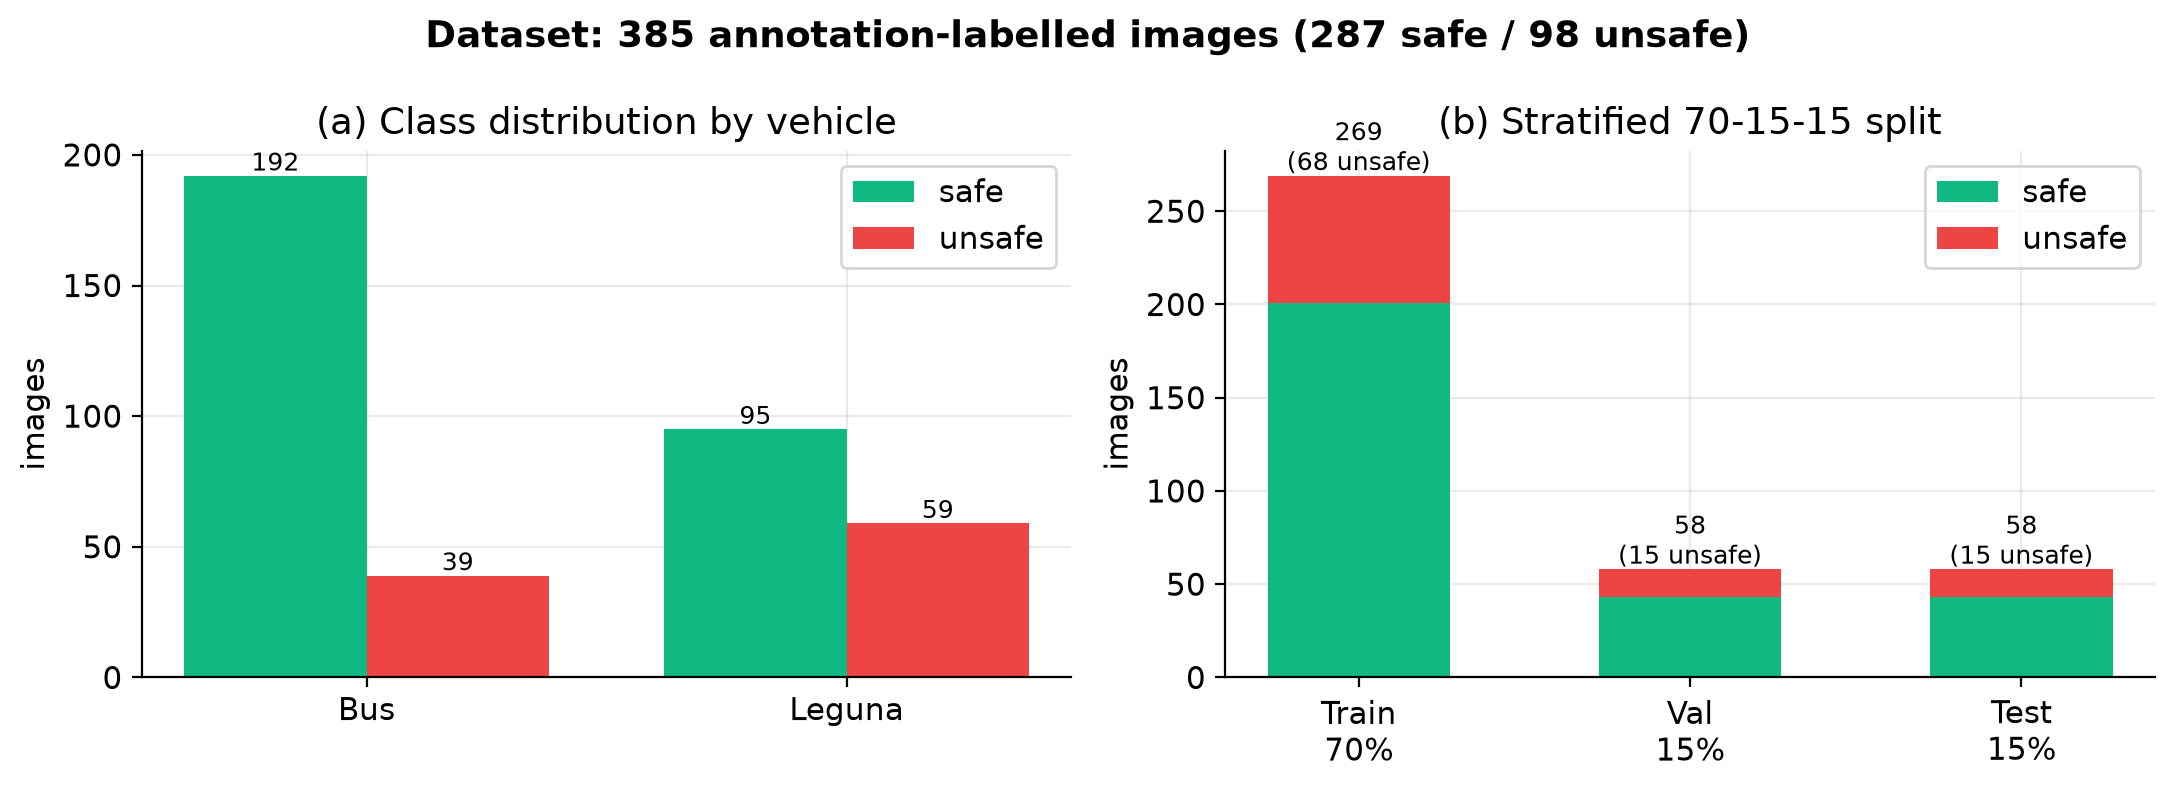
\includegraphics[width=\linewidth]{figures/fig1_dataset_overview.png}
    \caption{Updated dataset overview showing vehicle-wise class distribution and stratified 70/15/15 split composition.}
    \label{fig:eda}
\end{figure}

Representative examples of the vehicle categories are shown in Fig.~\ref{fig:leguna_samples} and Fig.~\ref{fig:bus_samples}.

\begin{figure}[!t]
    \centering
    \subfloat[Negative class.]{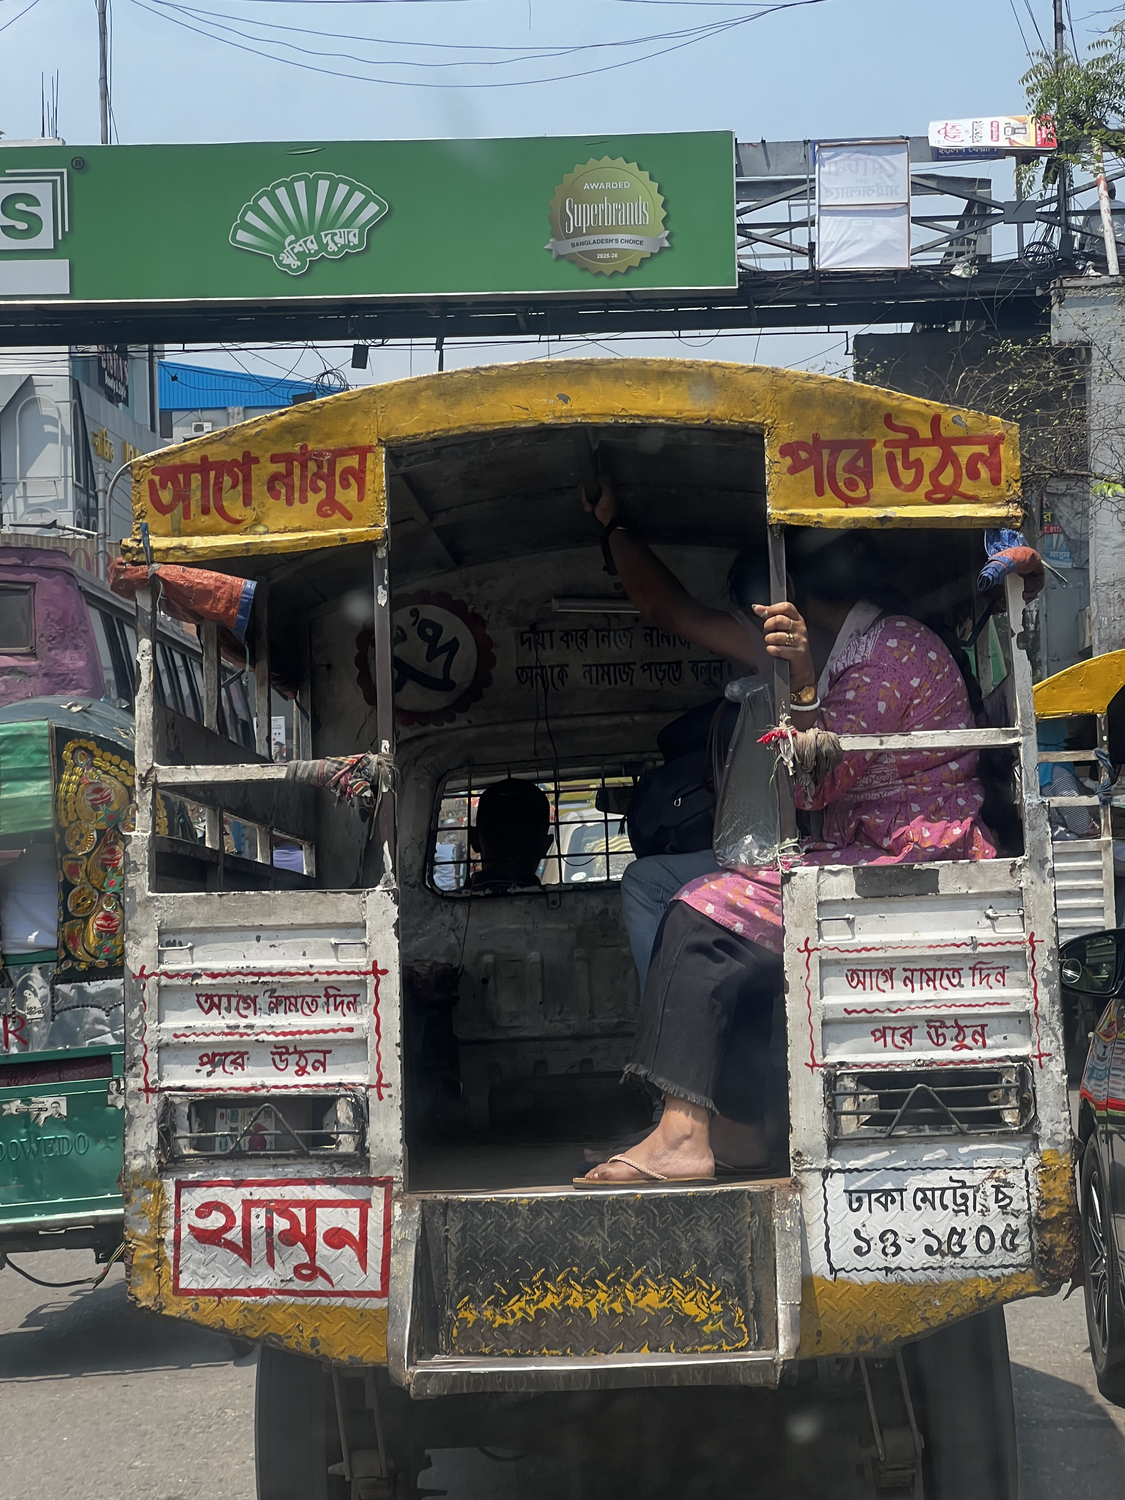
\includegraphics[width=0.4\linewidth]{leguna_negative.png}}
    \hfill
    \subfloat[Positive class.]{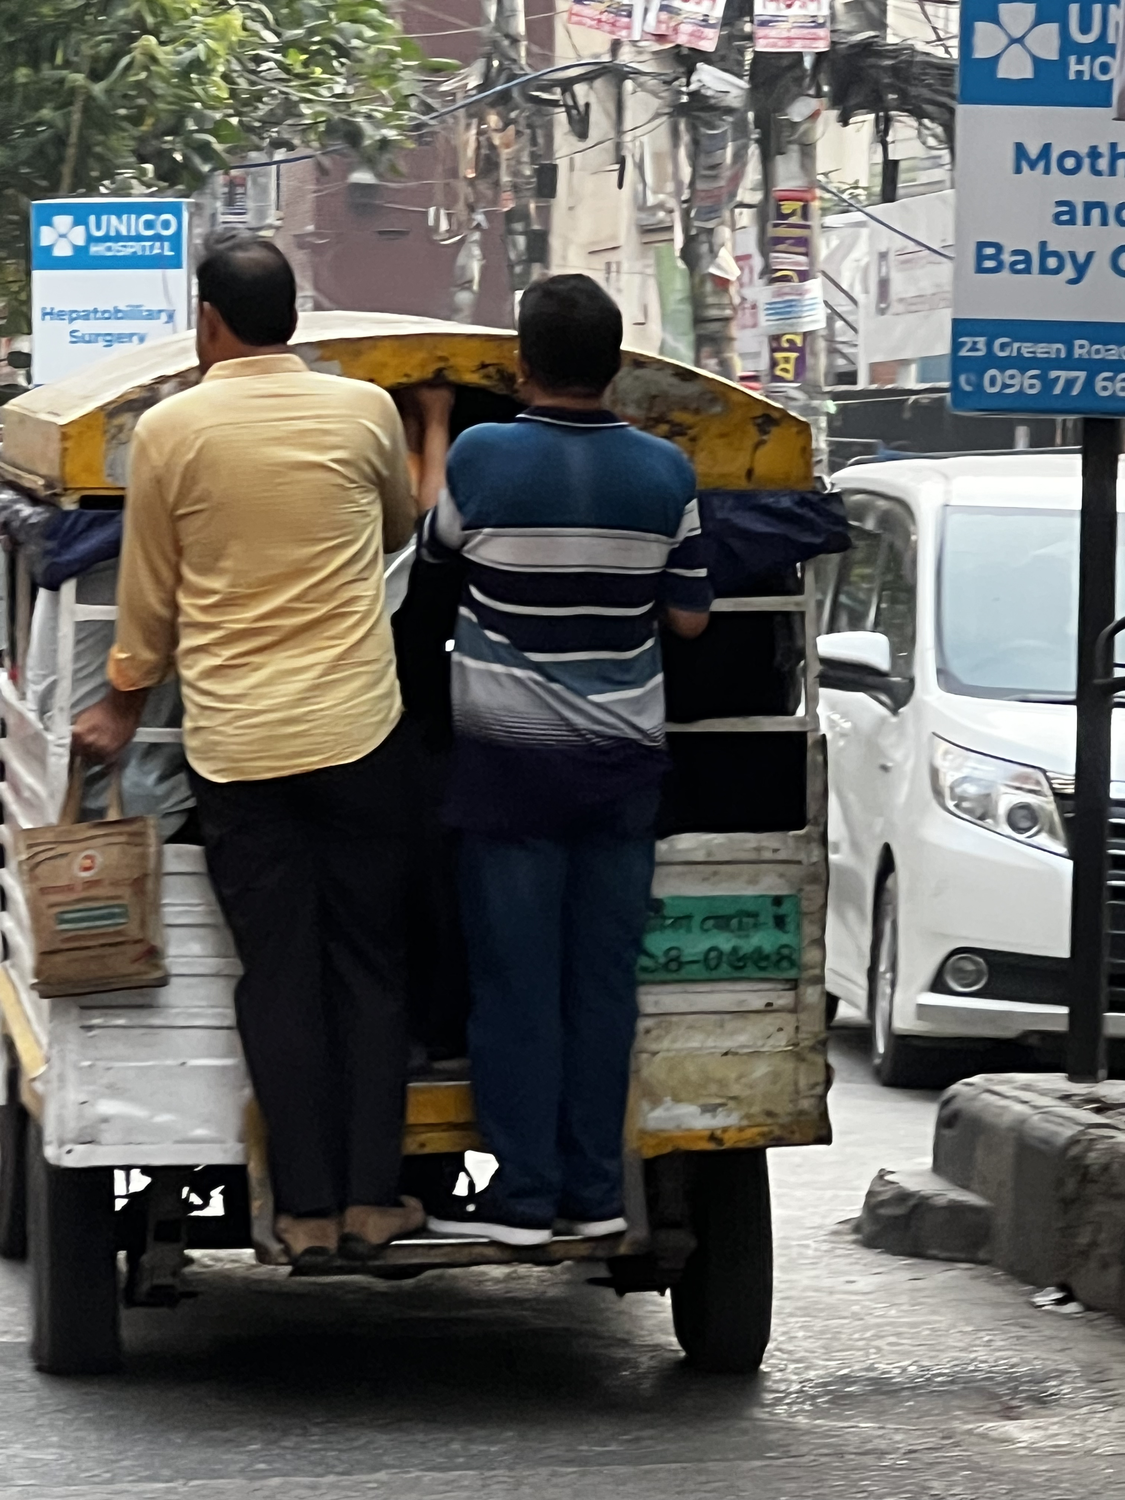
\includegraphics[width=0.4\linewidth]{leguna_positive.png}}
    \caption{Representative leguna samples.}
    \label{fig:leguna_samples}
\end{figure}

\begin{figure}[!t]
    \centering
    \subfloat[Negative class.]{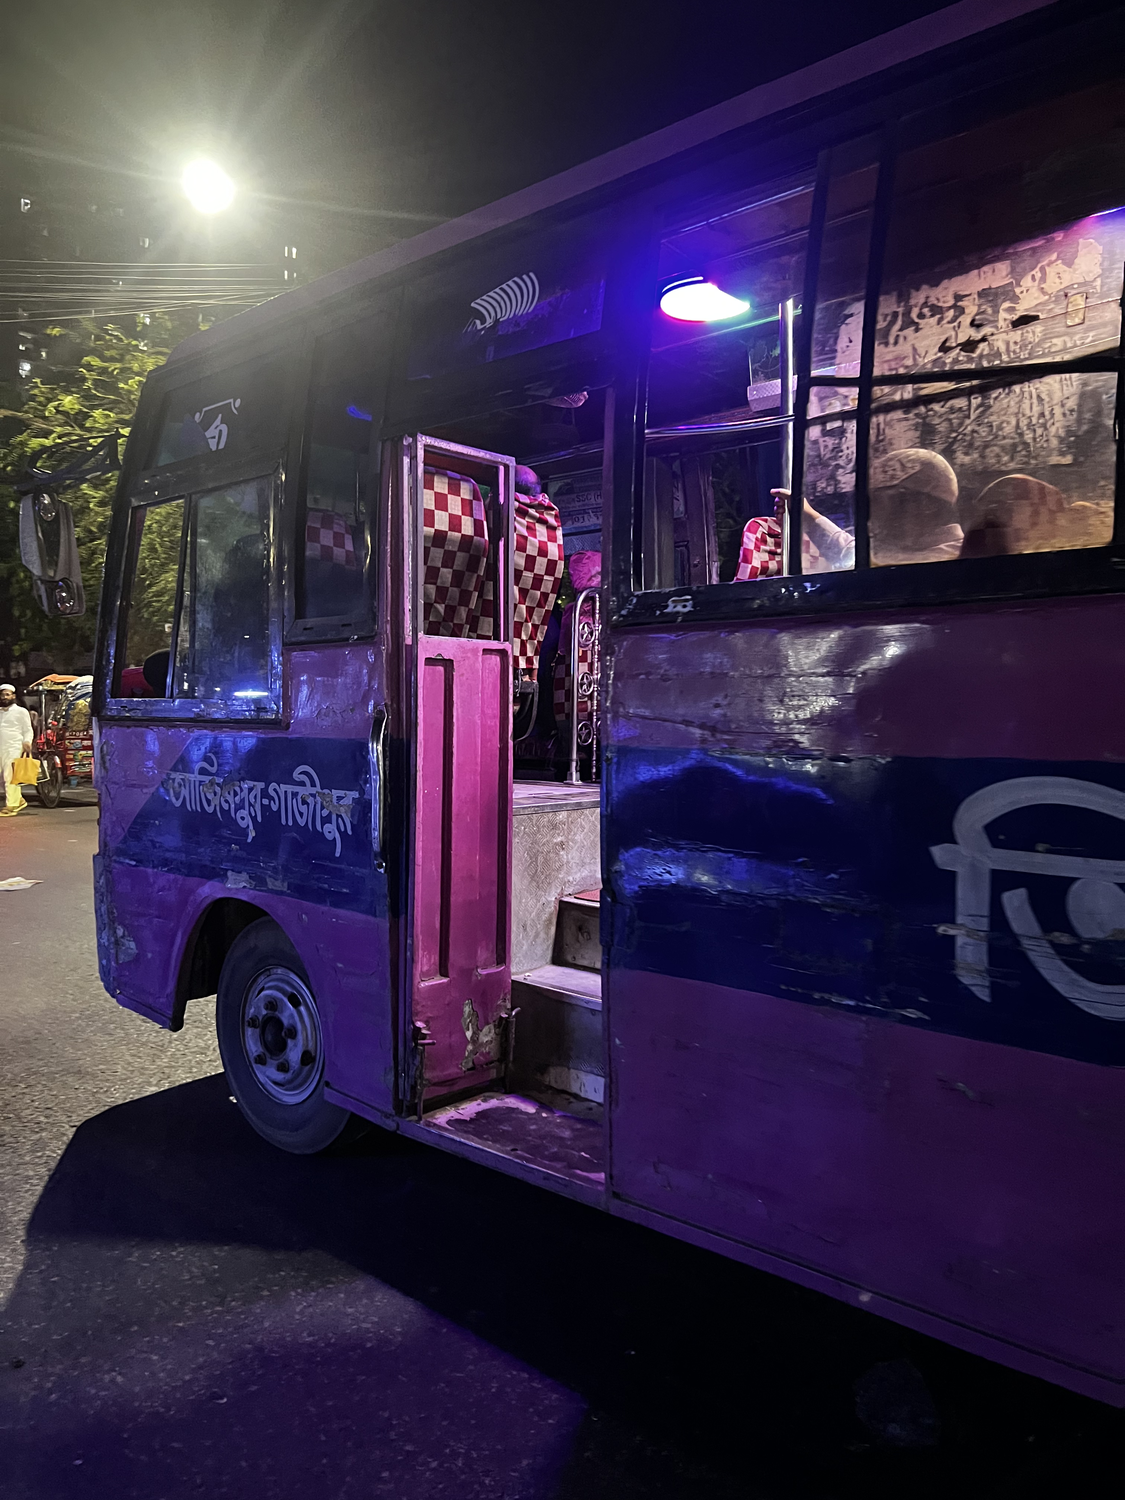
\includegraphics[width=0.4\linewidth]{bus_negative.png}}
    \hfill
    \subfloat[Positive class.]{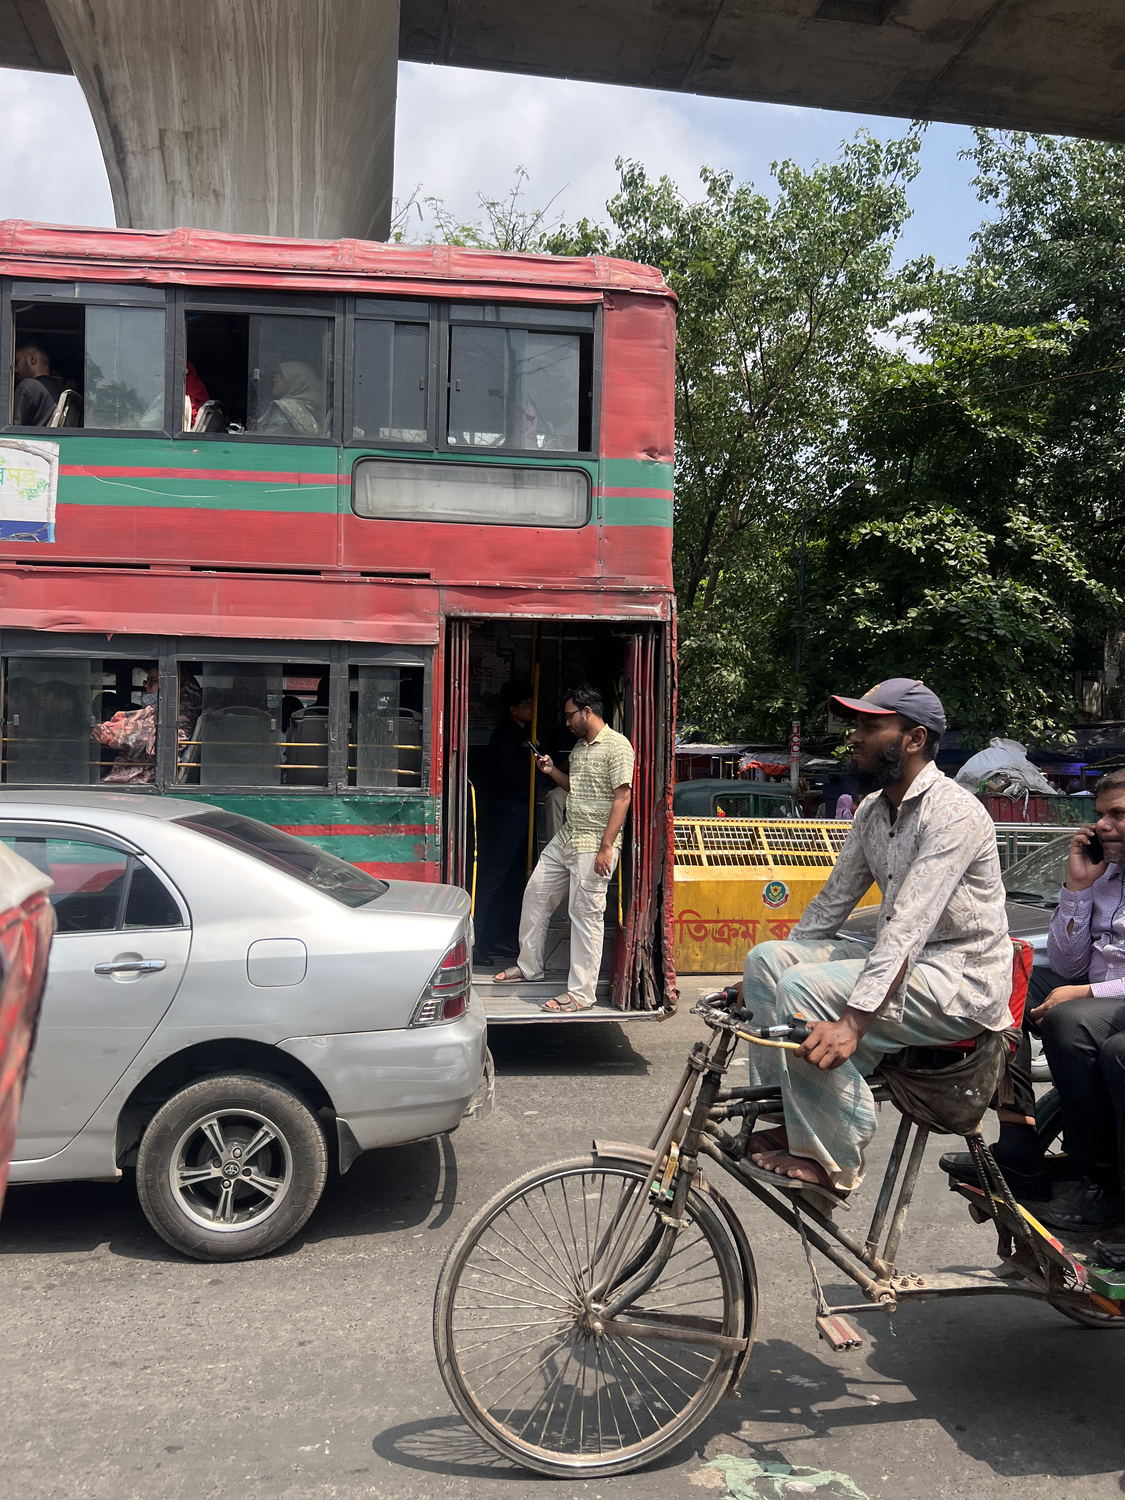
\includegraphics[width=0.4\linewidth]{bus_positive.png}}
    \caption{Representative bus samples.}
    \label{fig:bus_samples}
\end{figure}

\subsection{Data Cleaning}
Cleaning removed images whose content was blurred, ambiguous, low quality, heavily obstructed, poorly framed, or unreliable for class assignment. This step reduced label noise while preserving realistic variation in traffic, vehicle structure, crowding, and illumination.

\subsection{Data Annotation}
Manual annotation assigned each retained image to one of two classes: negative for safe/normal passenger conditions and positive for unsafe/risky hanging travel. Figure~\ref{fig:annotation_samples} shows representative annotation examples, including license-plate annotations retained only for possible future vehicle-identification integration.

\begin{figure}[!t]
    \centering
    \subfloat[Safe/normal annotation.]{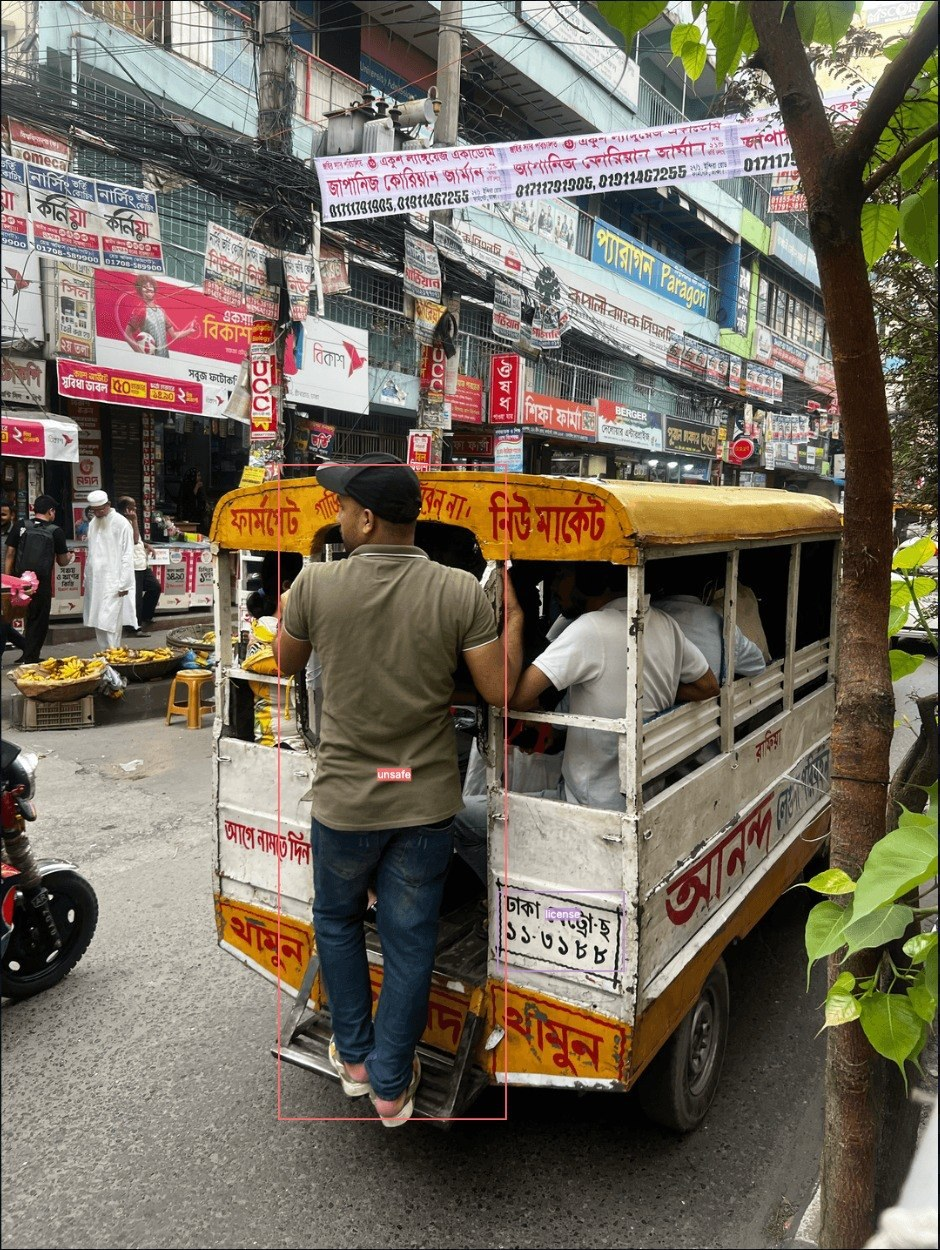
\includegraphics[width=0.35\linewidth]{annotation_1.jpeg}}
    \hfill
    \subfloat[Unsafe/risky annotation.]{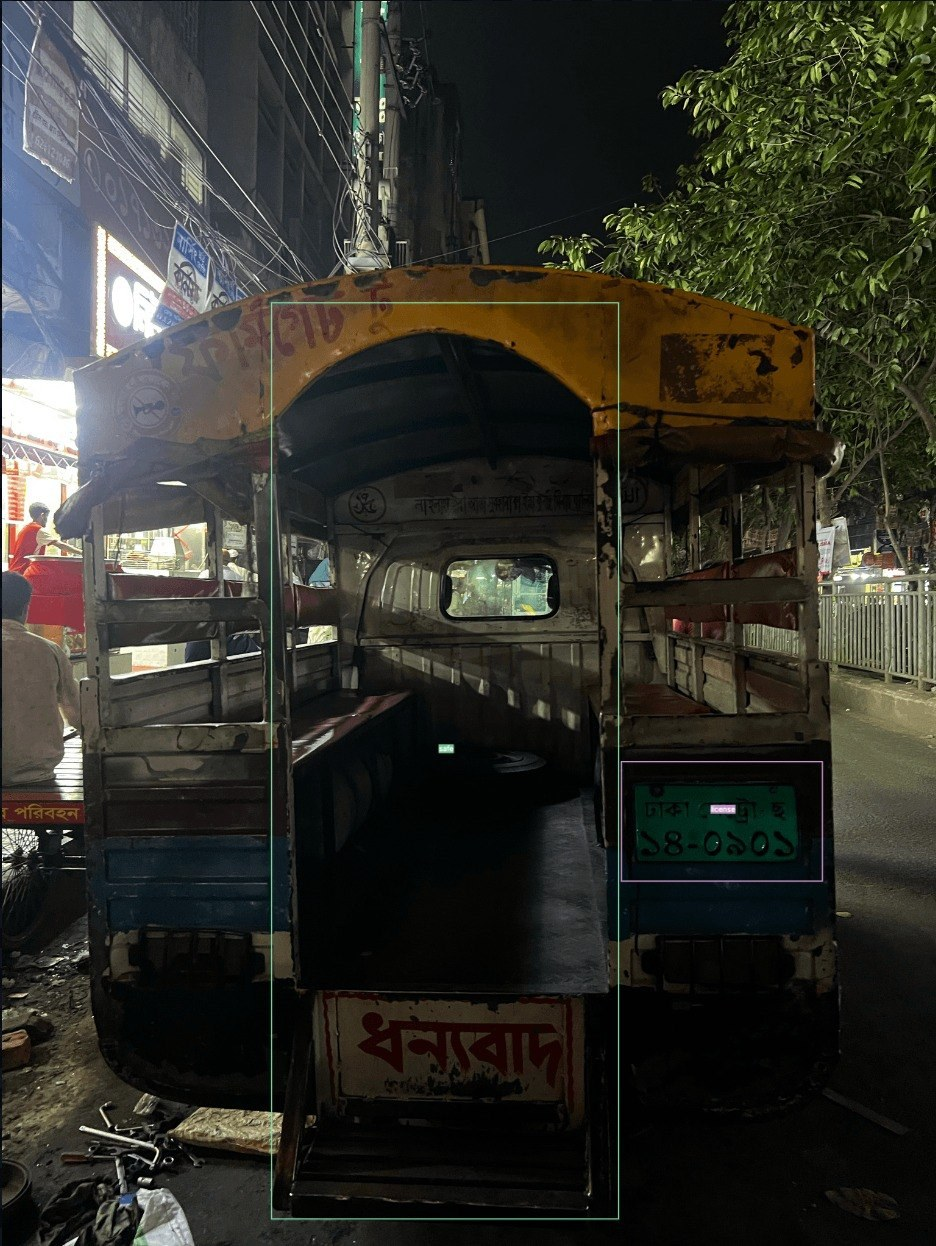
\includegraphics[width=0.35\linewidth]{annotation_2.jpeg}}

    \vspace{0.4cm}

    \subfloat[License-plate annotation.]{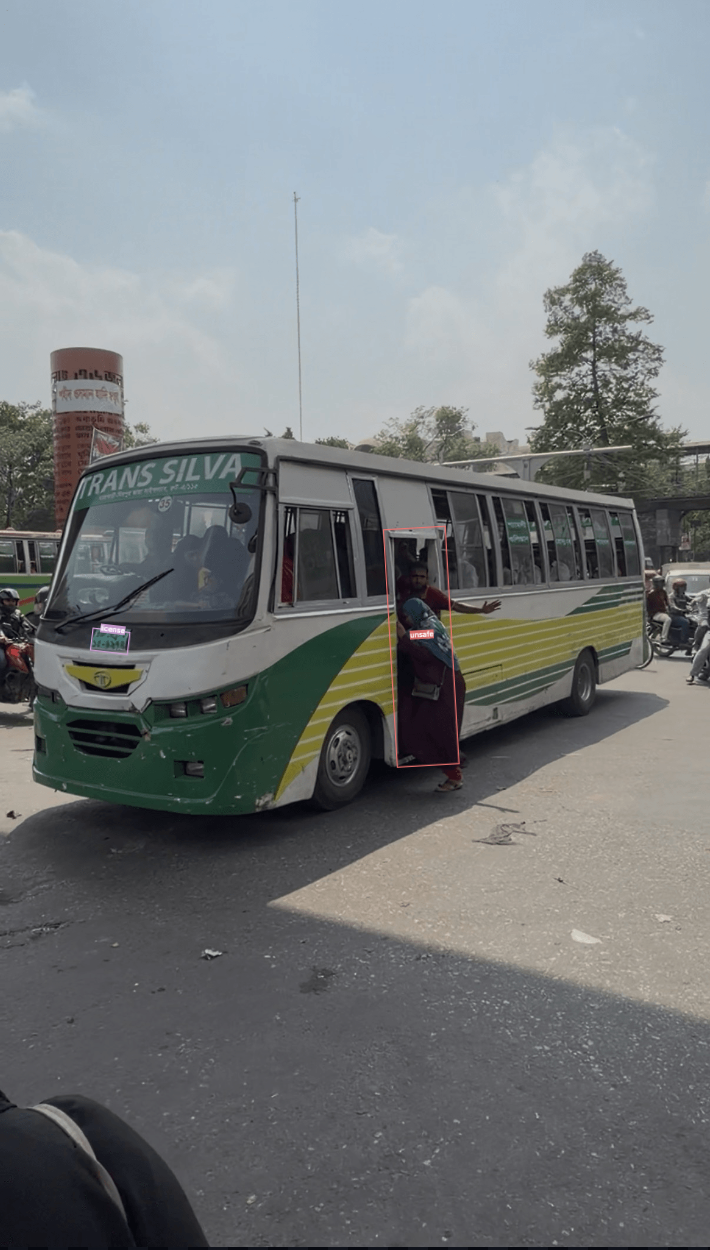
\includegraphics[width=0.35\linewidth]{annotation_3.png}}
    \hfill
    \subfloat[Combined annotation.]{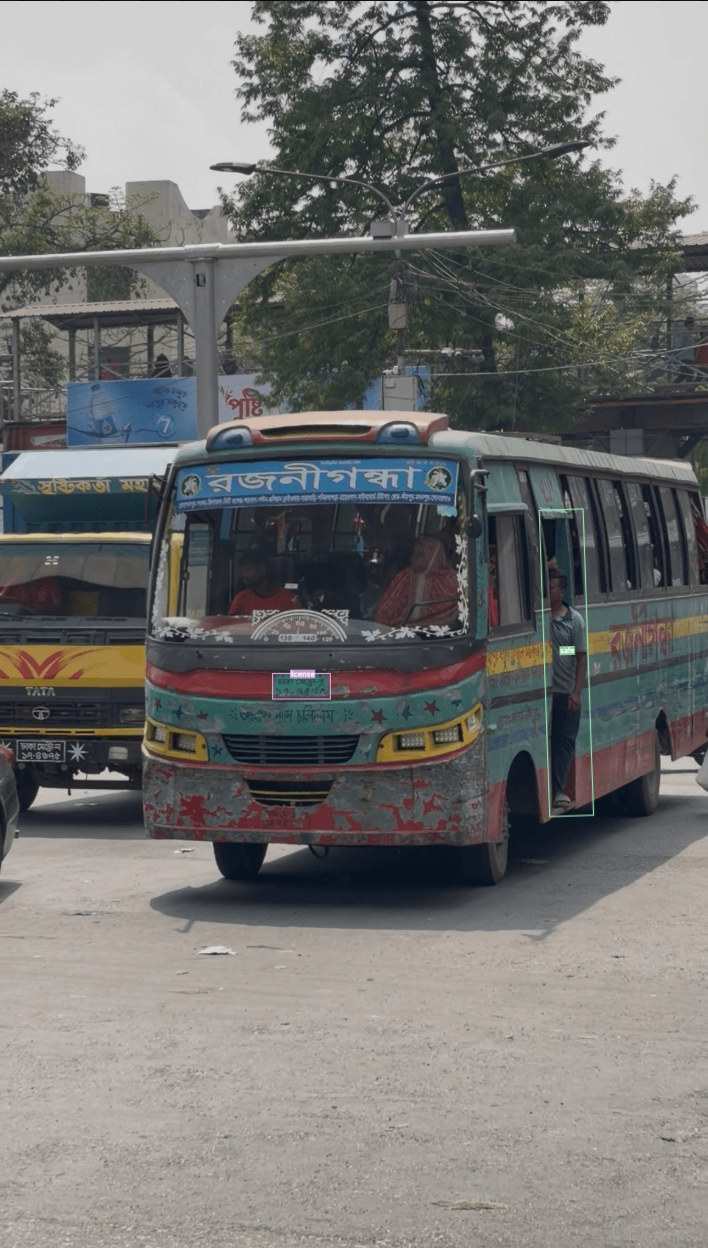
\includegraphics[width=0.35\linewidth]{annotation_4.png}}
    \caption{Representative annotation examples.}
    \label{fig:annotation_samples}
\end{figure}

\subsection{Data Augmentation}
Training-time augmentation was used to improve generalization without changing the held-out evaluation data. The updated experiments used task-aware augmentation, including conservative random resized cropping to preserve door-edge passengers, horizontal flipping, mild rotation, RandAugment, color jitter, and random erasing for deep models. HOG baselines used train-only offline augmentation. These transformations simulate common roadside imaging variation while preserving the class label \cite{shorten2019augmentation}.

All images were standardized before model-specific processing. The standardized preprocessing and model input settings are summarized in Table~\ref{tab:model_config}. The dataset is available online at \url{https://drive.google.com/drive/folders/1D3jDBvA-cAhwRPA4wUBUss5zlwdXdLJY}.

\subsection{Ethical Considerations}
The dataset is used only for academic safety-monitoring research. Images may contain privacy-sensitive visual information such as human faces, vehicle license plates, and location-related context. The classification task focuses on transport safety conditions rather than personal identity recognition; no face recognition, identity matching, or individual profiling is performed. Before any public release or operational deployment, privacy-preserving steps such as face and license-plate anonymization, removal of GPS or location metadata, consent and data-governance procedures, and compliance with relevant regulations would be required.

\section{Methodology}
The proposed method is a binary image-classification pipeline for public transport safety assessment. The workflow consists of dataset preparation, preprocessing, feature extraction or model-specific input preparation, model training, and evaluation. HOG-based classical models receive handcrafted gradient features, while deep neural models learn directly from image tensors. Implementation settings are summarized in Table~\ref{tab:model_config}.

\subsection{Pipeline Overview}
The pipeline begins with Dhaka bus and leguna image collection, followed by cleaning, annotation, augmentation, and standardization. Classical machine-learning models use HOG feature vectors extracted from grayscale inputs, whereas CNN and transfer-learning models receive RGB tensors. All models are evaluated on the same held-out split using standard classification metrics.

\begin{figure}[!t]
    \centering
    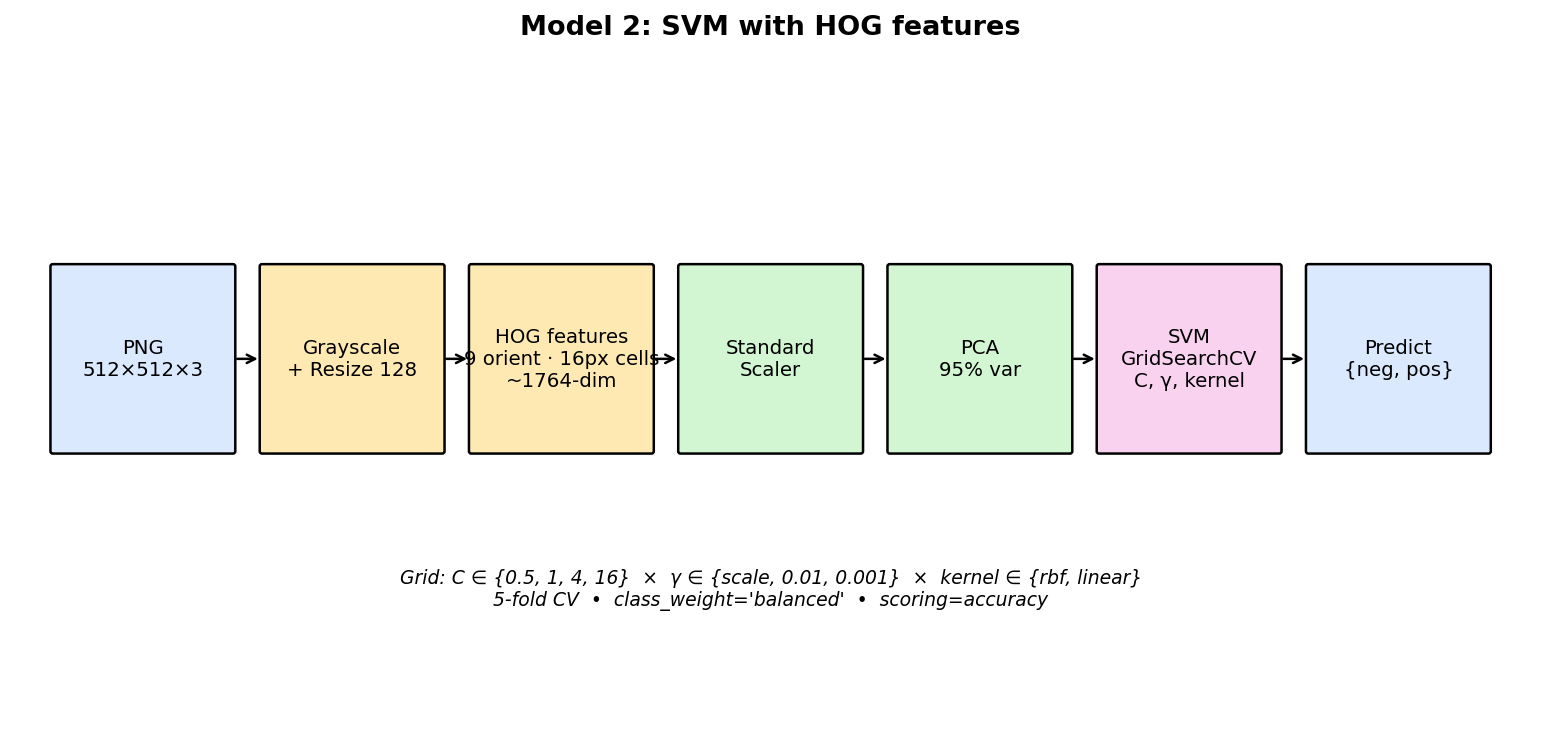
\includegraphics[width=\linewidth]{arch_svm.png}
    \caption{Overview of the HOG-based classical machine-learning pipeline.}
    \label{fig:arch_svm}
\end{figure}

\subsection{HOG-Based Feature Representation}
For the classical models, Histogram of Oriented Gradients (HOG) descriptors were extracted from grayscale images \cite{dalal2005hog}. HOG captures local gradient orientation and edge-structure information, which is useful for posture-, shape-, and boundary-related visual classification. Feature extraction was implemented with scikit-image \cite{vanderwalt2014skimage}; Table~\ref{tab:model_config} lists the extraction settings.

\subsection{Classical Machine Learning Models}
The classical baselines use HOG features with three complementary classifiers. Logistic Regression provides a linear probabilistic baseline and estimates the posterior probability of the positive class as
\[
P(y=1 \mid x) = \frac{1}{1 + e^{-w^{\top} x}} .
\]
The model is computationally efficient and interpretable, but its linear decision boundary can be limited when safe and unsafe samples are not linearly separable.

Gaussian Naive Bayes is a probabilistic baseline that assumes conditional independence among features given the class label. Each feature is modeled with a Gaussian likelihood,
\[
P(x_i \mid y) = \mathcal{N}(\mu_y, \sigma_y^2),
\]
and prediction is based on the posterior score
\[
P(y \mid x) \propto P(y) \prod_i P(x_i \mid y).
\]
Although the independence assumption is restrictive for correlated HOG features, the model is useful as a low-complexity comparator.

The Support Vector Machine (SVM) seeks a maximum-margin boundary between the negative and positive classes \cite{cortes1995svm}. The radial basis function (RBF) kernel handles non-linear separation in the HOG feature space through
\[
K(x_i, x_j) = \exp\!\left(-\gamma \lVert x_i - x_j \rVert^2\right).
\]
This kernel allows samples with similar HOG patterns to influence the decision function even when a linear boundary is insufficient. Table~\ref{tab:model_config} summarizes the implementation settings for all three classical models.

\subsection{Deep Neural Models}
The deep models process RGB images directly and learn spatial features from the training data \cite{krizhevsky2012alexnet}. The updated experiments evaluate five neural architectures: a CNN trained from scratch, ResNet18, EfficientNet-B0, ResNet50, and ConvNeXt-Tiny. The scratch CNN provides a lightweight learned-feature baseline, while ResNet18, EfficientNet-B0, ResNet50, and ConvNeXt-Tiny provide transfer-learning baselines with different depth, capacity, and convolutional design choices \cite{he2016resnet}, \cite{tan2019efficientnet}, \cite{liu2022convnext}. A probability-level ensemble combines the strongest transfer-learning models to improve ranking stability and support threshold-based safety modes. Weighted sampling, class-weighted loss, threshold tuning on out-of-fold probabilities, and horizontal-flip test-time augmentation were used to address class imbalance and improve unsafe-class recall. Figure~\ref{fig:arch_cnn} shows the CNN architecture, and Table~\ref{tab:model_config} reports the combined configuration.

\begin{figure}[!t]
    \centering
    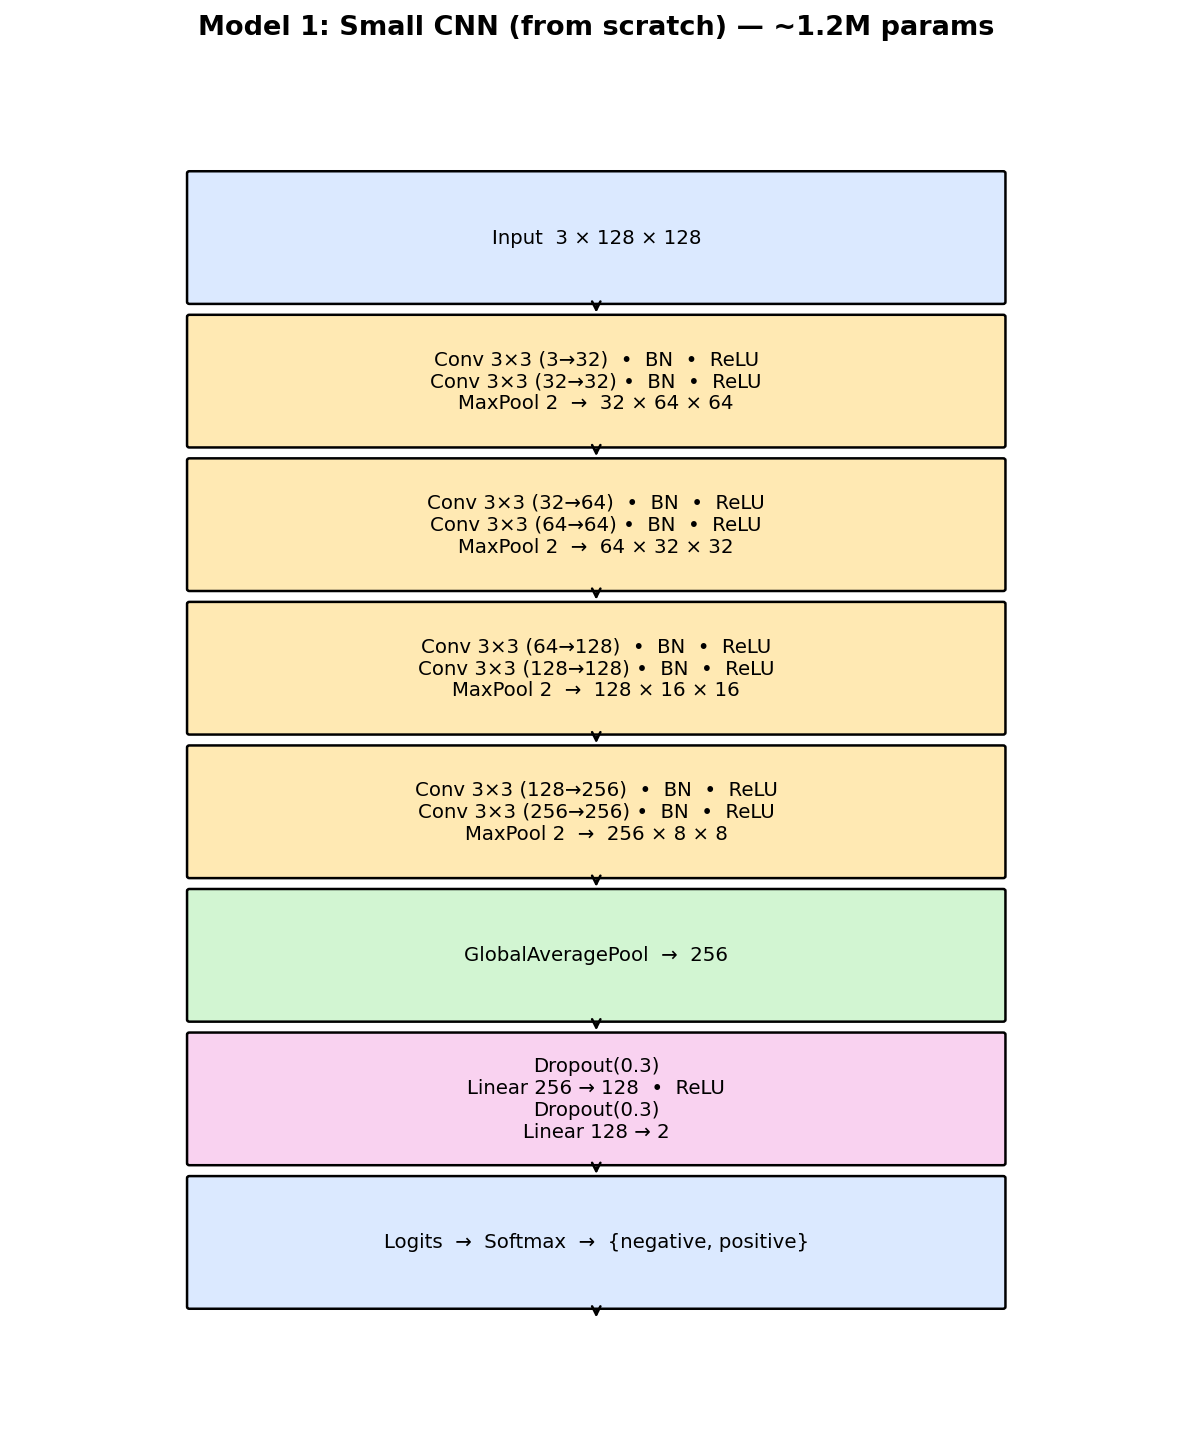
\includegraphics[width=\linewidth]{arch_cnn.png}
    \caption{CNN architecture used for image-level binary classification.}
    \label{fig:arch_cnn}
\end{figure}

\section{Experimental Setup}
\subsection{Split Protocol}
The data split followed a stratified, group-aware protocol to prevent augmented-data leakage. Images derived from the same source or augmentation group were kept within the same partition. Classical model hyperparameters were selected by cross-validation on the training set only, and the test set was reserved for final evaluation. Table~\ref{tab:model_config} gives the split and validation settings.

\subsection{Model Configuration}
The experiments were implemented in Python using scikit-learn for the classical pipelines \cite{pedregosa2011sklearn}, PyTorch for the neural model \cite{paszke2019pytorch}, and scikit-image for image processing \cite{vanderwalt2014skimage}. A fixed random seed of 42 was used for reproducibility. Model and preprocessing settings are consolidated in Table~\ref{tab:model_config}.

\begin{table*}[!t]
\centering
\caption{Model Configuration}
\label{tab:model_config}
\footnotesize
\begin{tabularx}{\textwidth}{l l X}
\toprule
\textbf{Model / Stage} & \textbf{Input Representation} & \textbf{Key Configuration} \\
\midrule
Image standardization & Source images & Orientation correction, RGB conversion, shorter side 512 px, center crop to $512\times512$, PNG output. \\
HOG feature extraction & Grayscale $128\times128$ & 9 orientation bins, $16\times16$ pixel cells, $2\times2$ cell blocks, L2-Hys normalization, 1764-d feature vector. \\
Logistic Regression & HOG features & StandardScaler, HOG feature vector, \texttt{lbfgs}, max iterations 2{,}000, $C=1.0$ in the updated classical baseline. \\
Gaussian Naive Bayes & HOG features & StandardScaler followed by Gaussian Naive Bayes; no tuned hyperparameters in the updated classical baseline. \\
SVM with RBF kernel & HOG features & StandardScaler, RBF kernel, $C=10$, $\gamma=\texttt{scale}$, probability estimates enabled. \\
CNN & RGB $128\times128$ & 4-block CNN trained from scratch; updated test metrics are included in the model comparison. \\
ResNet18 & RGB images & Transfer-learning baseline with residual blocks; evaluated on the held-out test set. \\
EfficientNet-B0 & RGB images & Transfer-learning baseline using compound scaling; included in both held-out test and 5-fold CV comparisons. \\
ResNet50 & RGB images, 320 px for CV & Deeper residual transfer-learning model; WeightedRandomSampler, class-weighted loss, out-of-fold threshold tuning, and horizontal-flip test-time augmentation for CV. \\
ConvNeXt-Tiny & RGB images, 320 px for CV & Modern convolutional transfer-learning model; same imbalance handling and test-time augmentation as ResNet50 in CV. \\
Ensemble & RGB $320\times320$ & Probability-level ensemble of ResNet50 and ConvNeXt-Tiny with selectable operating thresholds for balanced, high-recall, and zero-miss screening modes. \\
Evaluation protocol & Train/validation/test and CV & Stratified 70/15/15 split with 269 training, 58 validation, and 58 untouched test images; robust evaluation uses 5-fold stratified cross-validation on the 327 train+validation images. \\
\bottomrule
\end{tabularx}
\end{table*}

For HOG-based models, preprocessing and dimensionality-reduction steps were fitted on the training data and then applied to validation folds and the test set. The CNN used normalized RGB image tensors rather than HOG descriptors.

For CNN inference, logits $z \in \mathbb{R}^{2}$ are converted to class probabilities by
\[
p_k = \frac{e^{z_k}}{\sum_{j=0}^{1} e^{z_j}}, \qquad k \in \{0, 1\}.
\]
The optimizer and learning-rate schedule are listed in Table~\ref{tab:model_config} \cite{kingma2015adam}.

\subsection{Evaluation Metrics}
Evaluation used accuracy, precision, recall, F1-score, confusion matrices, and AUC. Learning curves were used where applicable to inspect neural-model training behavior. Let $TP$, $TN$, $FP$, and $FN$ denote true positives, true negatives, false positives, and false negatives, with the positive class corresponding to unsafe/risky hanging travel. The scalar metrics are
\begin{align*}
\mathrm{Accuracy} & = \frac{TP + TN}{TP + TN + FP + FN}, \\
\mathrm{Precision} & = \frac{TP}{TP + FP}, \qquad
\mathrm{Recall} = \frac{TP}{TP + FN},
\end{align*}
\[
F_1 = 2 \cdot \frac{\mathrm{Precision} \cdot \mathrm{Recall}}{\mathrm{Precision} + \mathrm{Recall}}.
\]
Because missed unsafe cases have direct safety implications, positive-class recall is considered alongside overall accuracy and AUC.


\section{Results}
\subsection{Quantitative Comparison}
This section reports the updated results. Table~\ref{tab:test_results} gives the full held-out test comparison from the supplied CSV file, while Table~\ref{tab:cv_results} reports the more reliable 5-fold cross-validation metrics for the deep models from the supplied CV table. The untouched 58-image holdout contains only about 15 unsafe samples, so cross-validation over the 327 train+validation images is used for the headline deep-model conclusion. The ResNet50--ConvNeXt ensemble gives the strongest balanced cross-validated performance overall, while SVM remains the strongest classical HOG baseline by AUC.

\begin{table*}[!t]
\centering
\caption{Held-out Test Performance for All Reported Models}
\label{tab:test_results}
\footnotesize
\setlength{\tabcolsep}{3pt}
\resizebox{\textwidth}{!}{%
\begin{tabular}{l l l r c c c c c c c}
\toprule
\textbf{Model} & \textbf{Family} & \textbf{Dev.} & \textbf{Params} & \textbf{Acc.} & \textbf{Unsafe R} & \textbf{Unsafe P} & \textbf{F1} & \textbf{AUC} & \textbf{AP} & \textbf{MCC} \\
\midrule
Logistic Regression & Classical & CPU & -- & 0.707 & 0.733 & 0.458 & 0.564 & 0.822 & 0.745 & 0.383 \\
Naive Bayes & Classical & CPU & -- & 0.672 & 0.600 & 0.409 & 0.486 & 0.698 & 0.578 & 0.269 \\
SVM (RBF) & Classical & CPU & -- & 0.793 & 0.667 & 0.588 & 0.625 & 0.836 & 0.762 & 0.485 \\
CNN & CNN-scratch & GPU & 1{,}206{,}370 & \textbf{0.914} & 0.667 & \textbf{1.000} & \textbf{0.800} & 0.822 & 0.823 & \textbf{0.773} \\
ResNet18 & Transfer & GPU & 11{,}177{,}538 & 0.862 & 0.667 & 0.769 & 0.714 & 0.826 & 0.812 & 0.627 \\
EfficientNet-B0 & Transfer & GPU & 4{,}010{,}110 & 0.828 & 0.733 & 0.647 & 0.688 & 0.864 & 0.819 & 0.571 \\
ResNet50 & Transfer & GPU & 23{,}512{,}130 & 0.828 & \textbf{0.800} & 0.632 & 0.706 & 0.885 & \textbf{0.847} & 0.595 \\
ConvNeXt-Tiny & Transfer & GPU & 27{,}821{,}666 & 0.862 & 0.667 & 0.769 & 0.714 & \textbf{0.907} & 0.837 & 0.627 \\
Ensemble (best) & Ensemble & GPU & -- & 0.845 & 0.667 & 0.714 & 0.690 & 0.901 & 0.837 & 0.587 \\
\bottomrule
\end{tabular}
}
\end{table*}

\begin{table}[!t]
\centering
\caption{Cross-Validated Deep-Model Metrics}
\label{tab:cv_results}
\footnotesize
\setlength{\tabcolsep}{2pt}
\resizebox{\linewidth}{!}{%
\begin{tabular}{lccccccc}
\toprule
\textbf{Model} & \textbf{Acc.} & \textbf{Unsafe R} & \textbf{Unsafe P} & \textbf{F1} & \textbf{AUC} & \textbf{AP} & \textbf{MCC} \\
\midrule
ResNet50 & 0.905 & \textbf{0.843} & 0.795 & 0.819 & 0.919 & 0.879 & 0.755 \\
ConvNeXt-Tiny & 0.905 & 0.819 & 0.810 & 0.814 & 0.923 & 0.874 & 0.751 \\
EfficientNet-B0 & 0.865 & 0.783 & 0.714 & 0.747 & 0.884 & 0.820 & 0.657 \\
Ensemble (best) & \textbf{0.917} & 0.807 & \textbf{0.859} & \textbf{0.832} & \textbf{0.929} & \textbf{0.883} & \textbf{0.778} \\
\bottomrule
\end{tabular}
}
\end{table}

\begin{figure*}[!t]
    \centering
    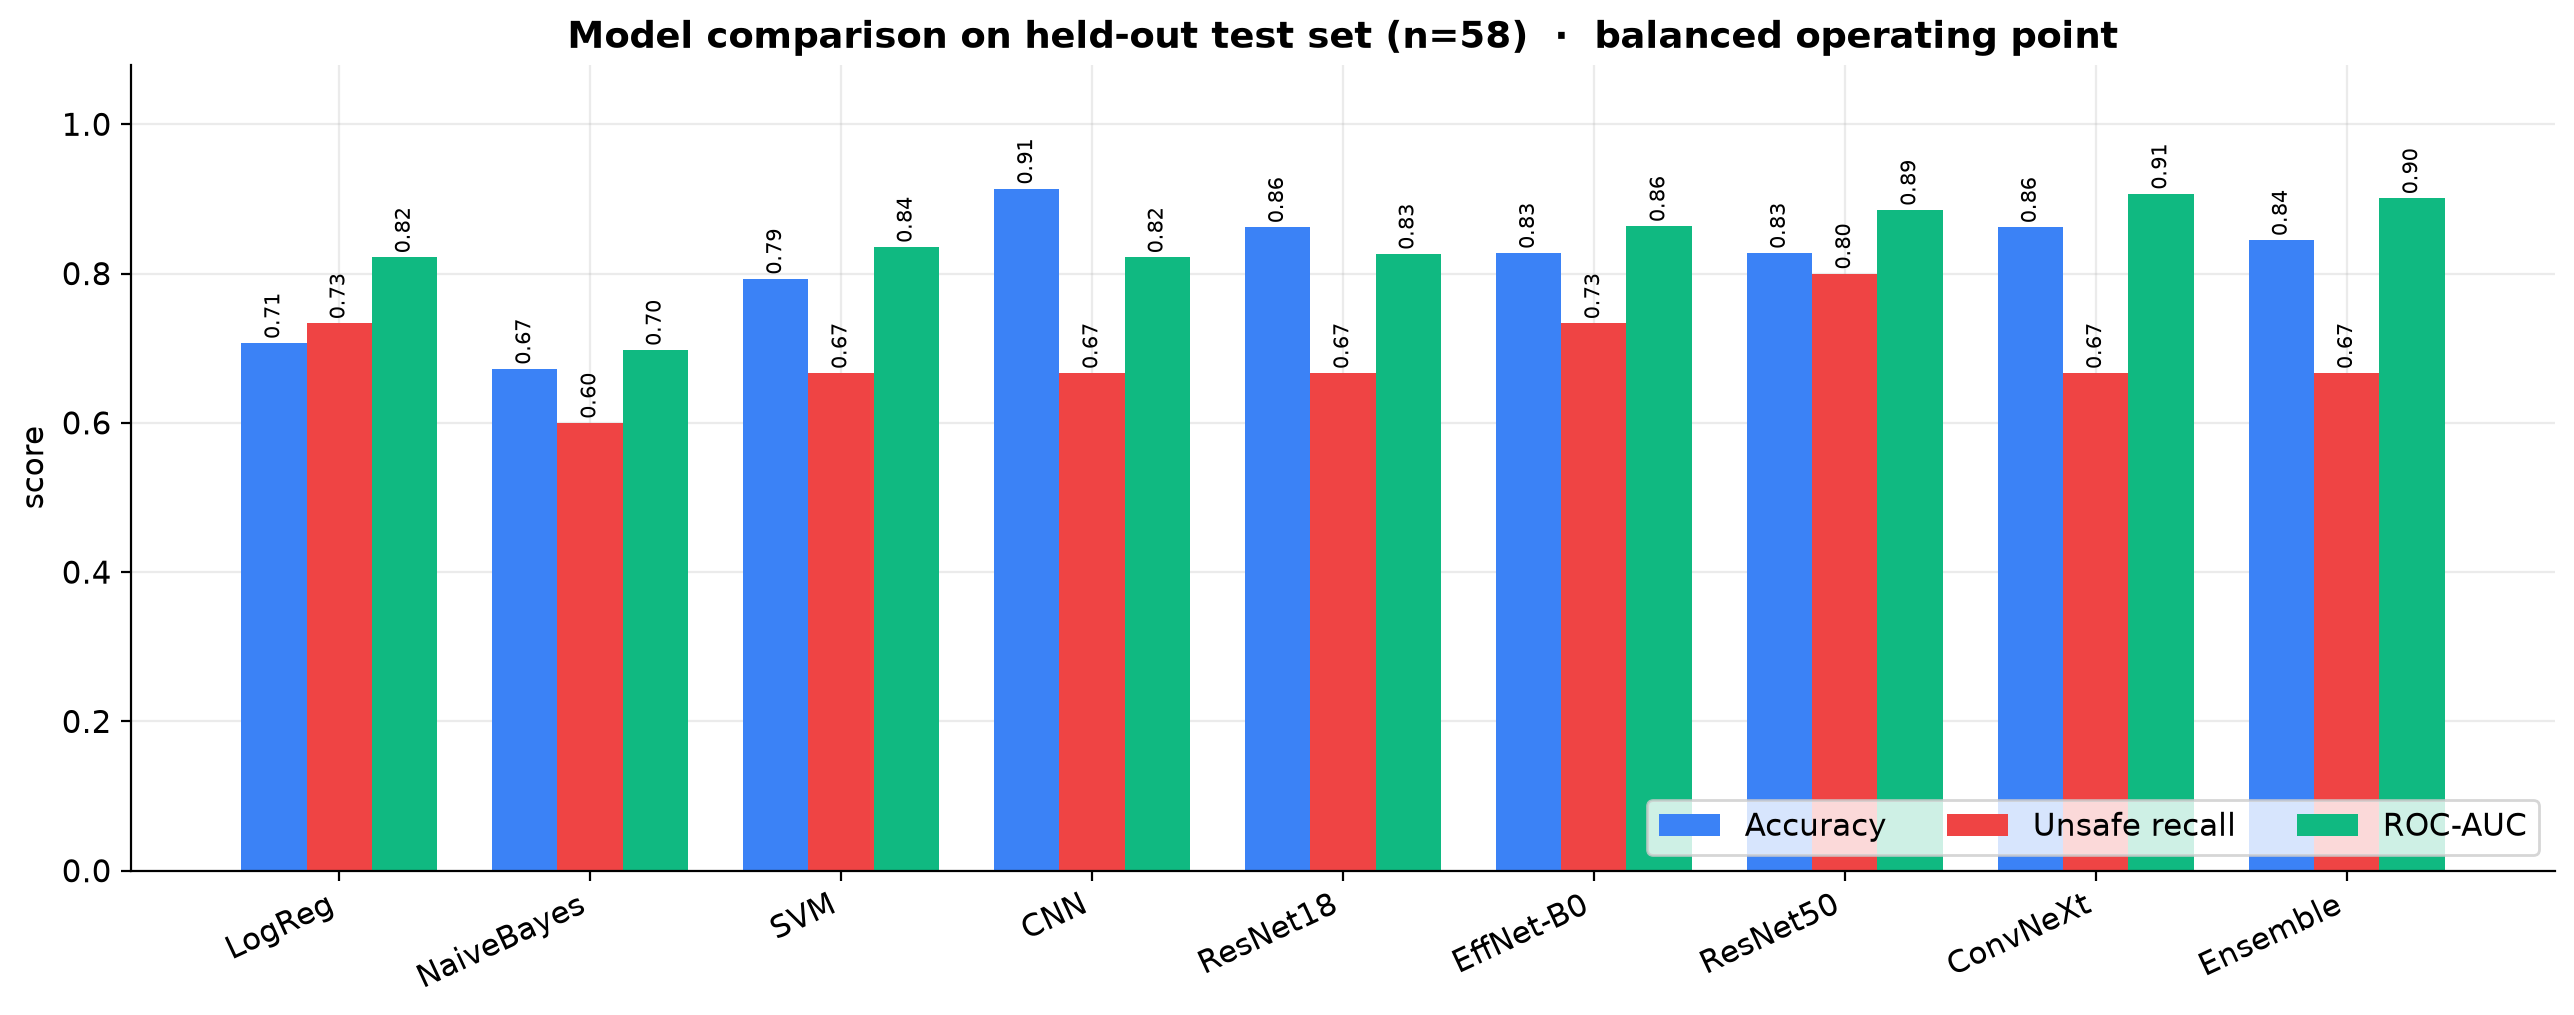
\includegraphics[width=\textwidth]{figures/fig2_model_comparison.png}
    \caption{Held-out test comparison of accuracy, unsafe recall, and ROC-AUC across all nine reported models.}
    \label{fig:paper_model_comparison}
\end{figure*}

\begin{table}[!t]
\centering
\caption{Selectable operating points for the deployed ensemble.}
\label{tab:operating_modes}
\small
\setlength{\tabcolsep}{4pt}
\begin{tabular}{lcccc}
\toprule
\textbf{Mode} & \textbf{Threshold} & \textbf{CV Acc.} & \textbf{Unsafe R} & \textbf{Unsafe P} \\
\midrule
Balanced & 0.570 & 0.917 & 0.807 & 0.859 \\
High recall & 0.125 & 0.746 & 0.952 & 0.500 \\
Zero miss & 0.017 & 0.260 & 1.000 & 0.255 \\
\bottomrule
\end{tabular}
\end{table}

\begin{figure}[!t]
    \centering
    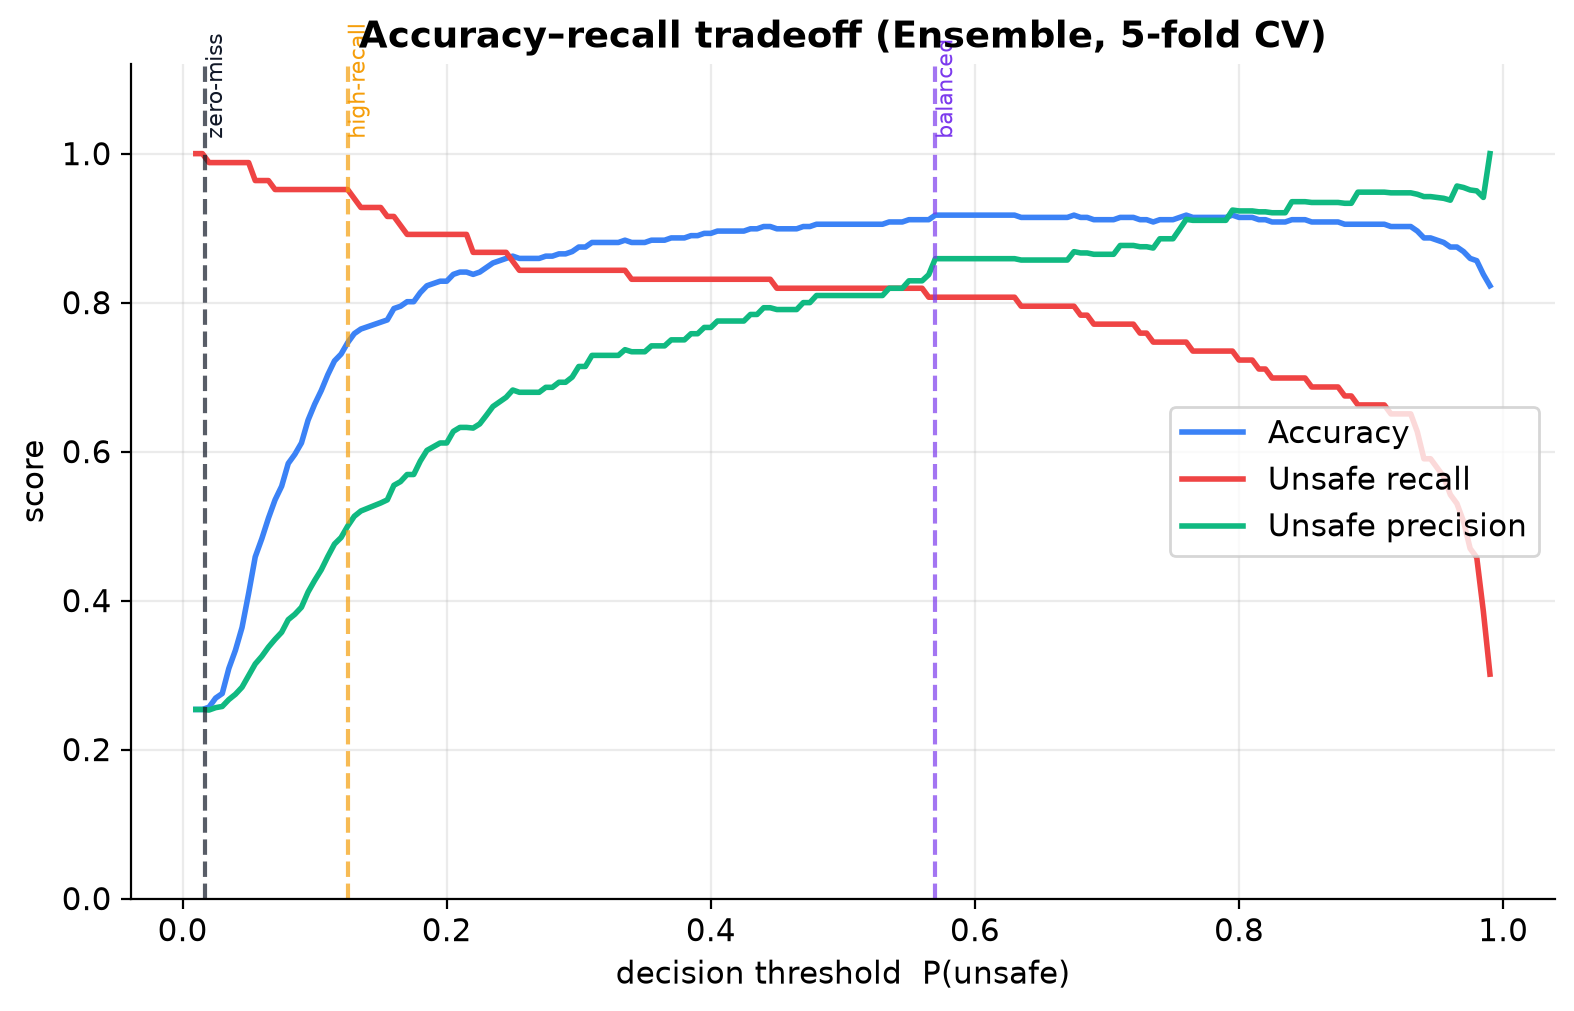
\includegraphics[width=\linewidth]{figures/fig6_tradeoff.png}
    \caption{Accuracy, unsafe recall, and precision tradeoff for the ensemble threshold, including the deployed operating modes.}
    \label{fig:paper_tradeoff}
\end{figure}

\subsection{Confusion Matrix Analysis}
The confusion matrices in Fig.~\ref{fig:paper_confusion_matrices} report class-level outcomes for all nine models on the held-out test set. The rows show true labels and the columns show predicted labels, with safe representing normal passenger conditions and unsafe representing door-hanging risk.

\begin{figure*}[!t]
    \centering
    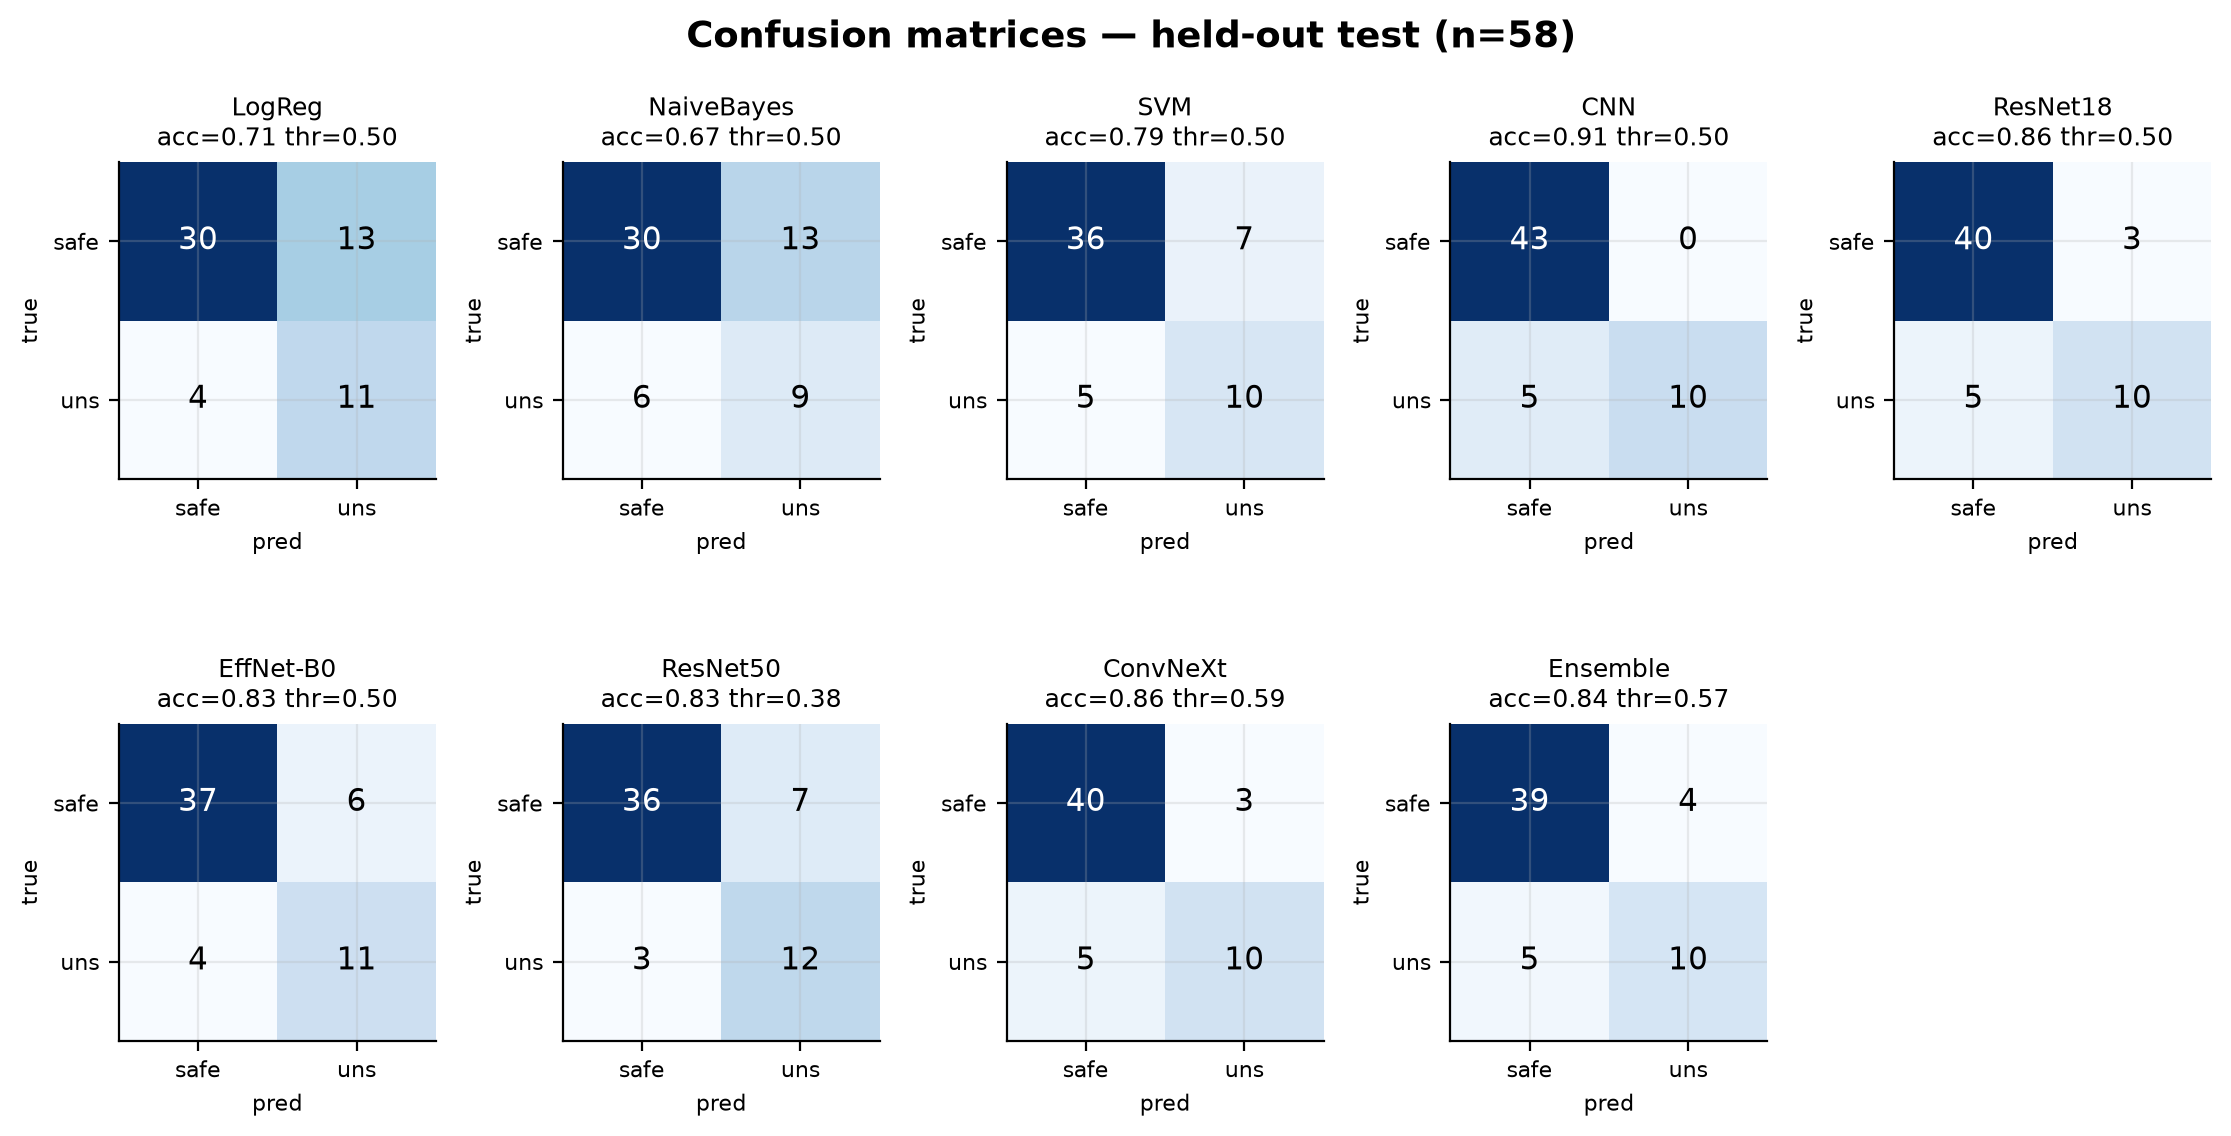
\includegraphics[width=\textwidth]{figures/fig5_confusion_matrices.png}
    \caption{Confusion-matrix grid for all nine reported models on the held-out test set.}
    \label{fig:paper_confusion_matrices}
\end{figure*}

\subsection{ROC and AUC Analysis}
AUC values are reported in Tables~\ref{tab:test_results} and~\ref{tab:cv_results}. Figure~\ref{fig:paper_roc_test} shows held-out ROC curves for all reported models, Fig.~\ref{fig:paper_pr_curves} shows the corresponding precision--recall curves, and Fig.~\ref{fig:paper_roc_cv_deep} shows the more reliable 5-fold cross-validated ROC curves for the deep models.

\begin{figure*}[!t]
    \centering
    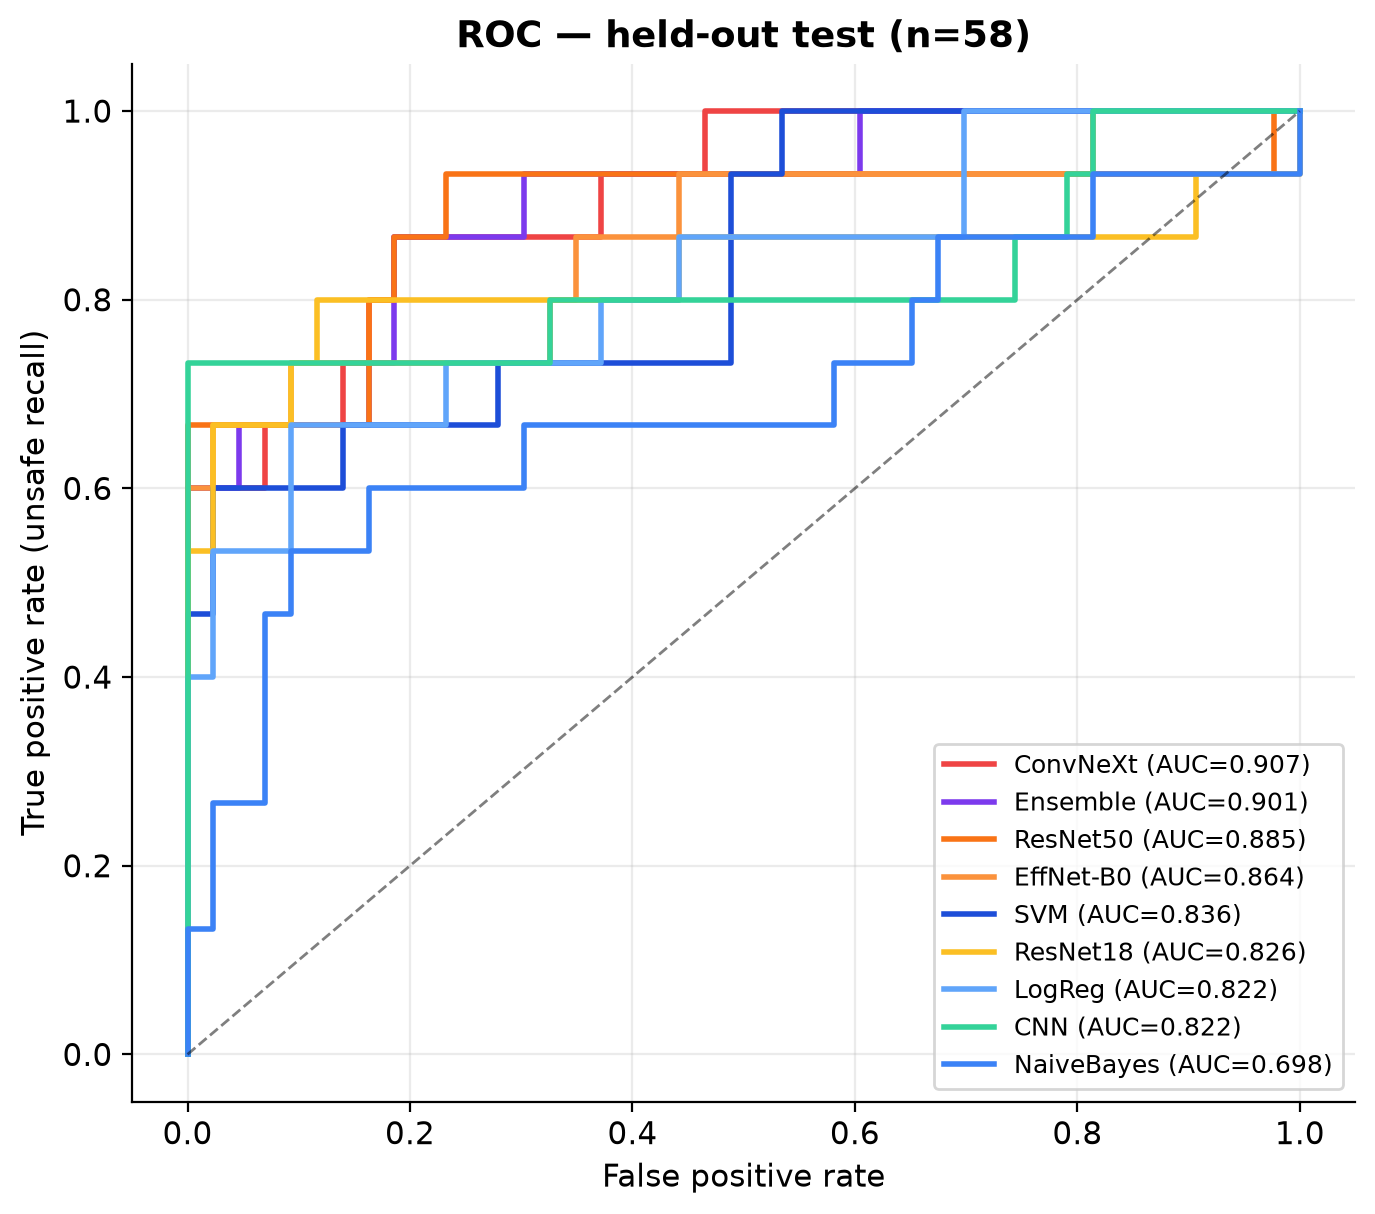
\includegraphics[width=0.72\textwidth]{figures/fig3b_roc_test.png}
    \caption{ROC curves for all nine reported models on the held-out test set.}
    \label{fig:paper_roc_test}
\end{figure*}

\begin{figure*}[!t]
    \centering
    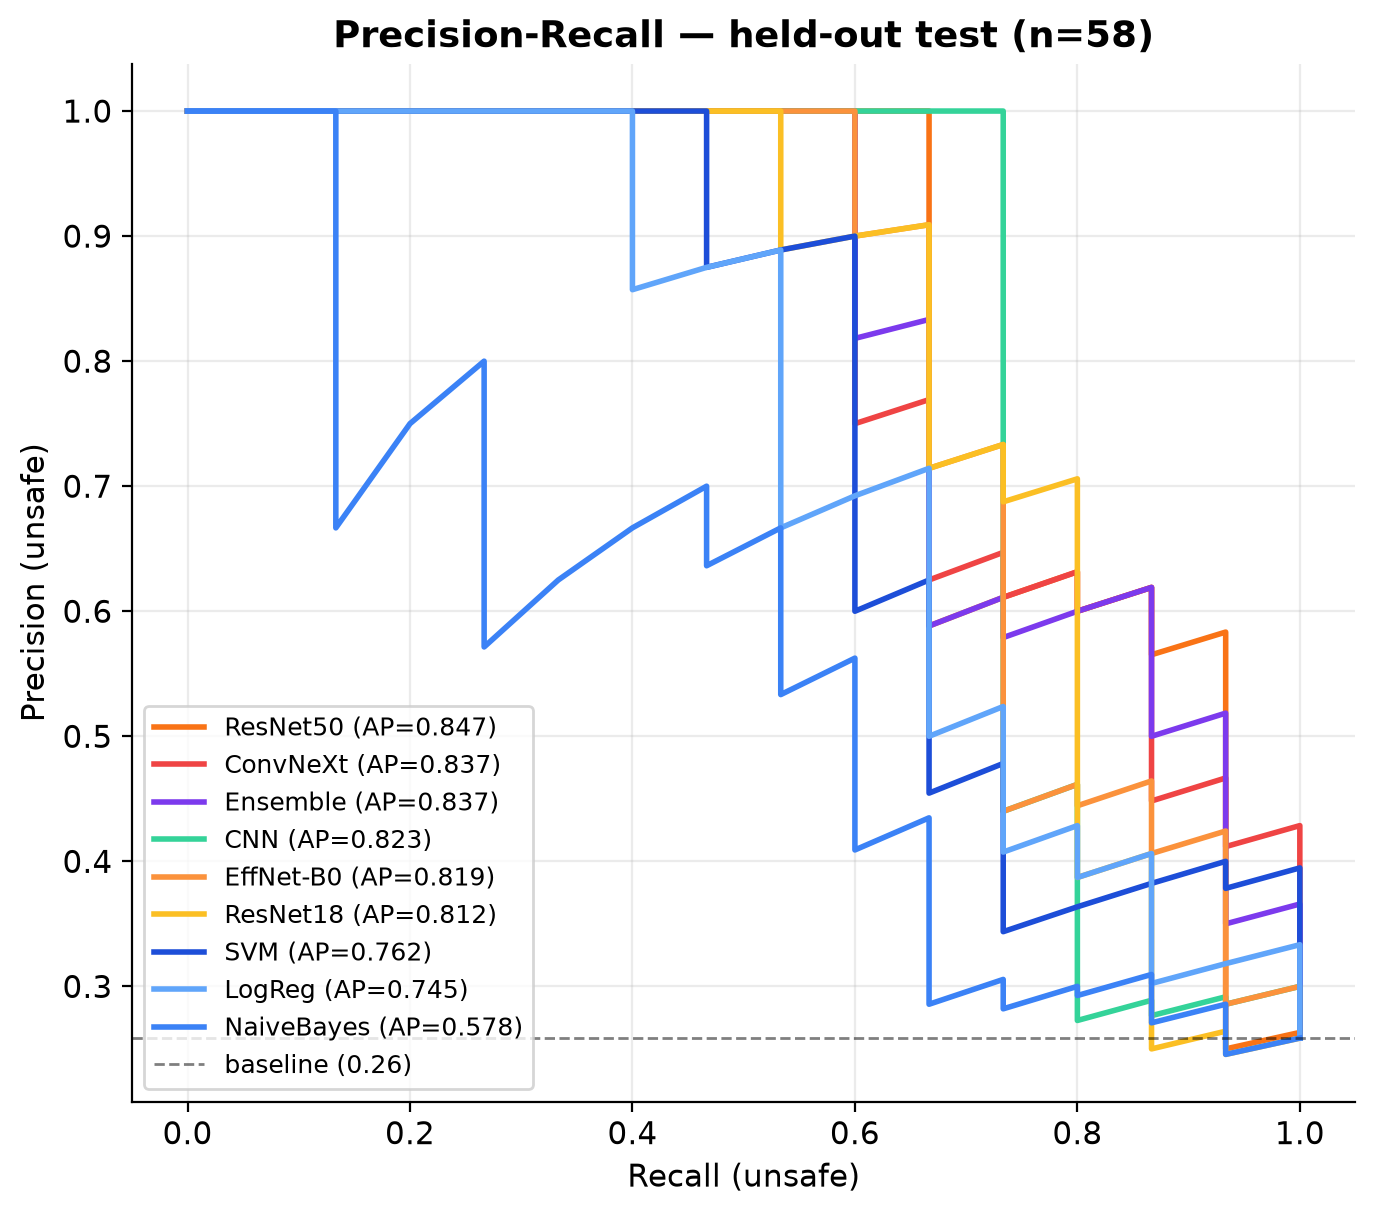
\includegraphics[width=0.72\textwidth]{figures/fig4_pr_curves.png}
    \caption{Precision--recall curves for all nine reported models on the held-out test set.}
    \label{fig:paper_pr_curves}
\end{figure*}

\begin{figure}[!t]
    \centering
    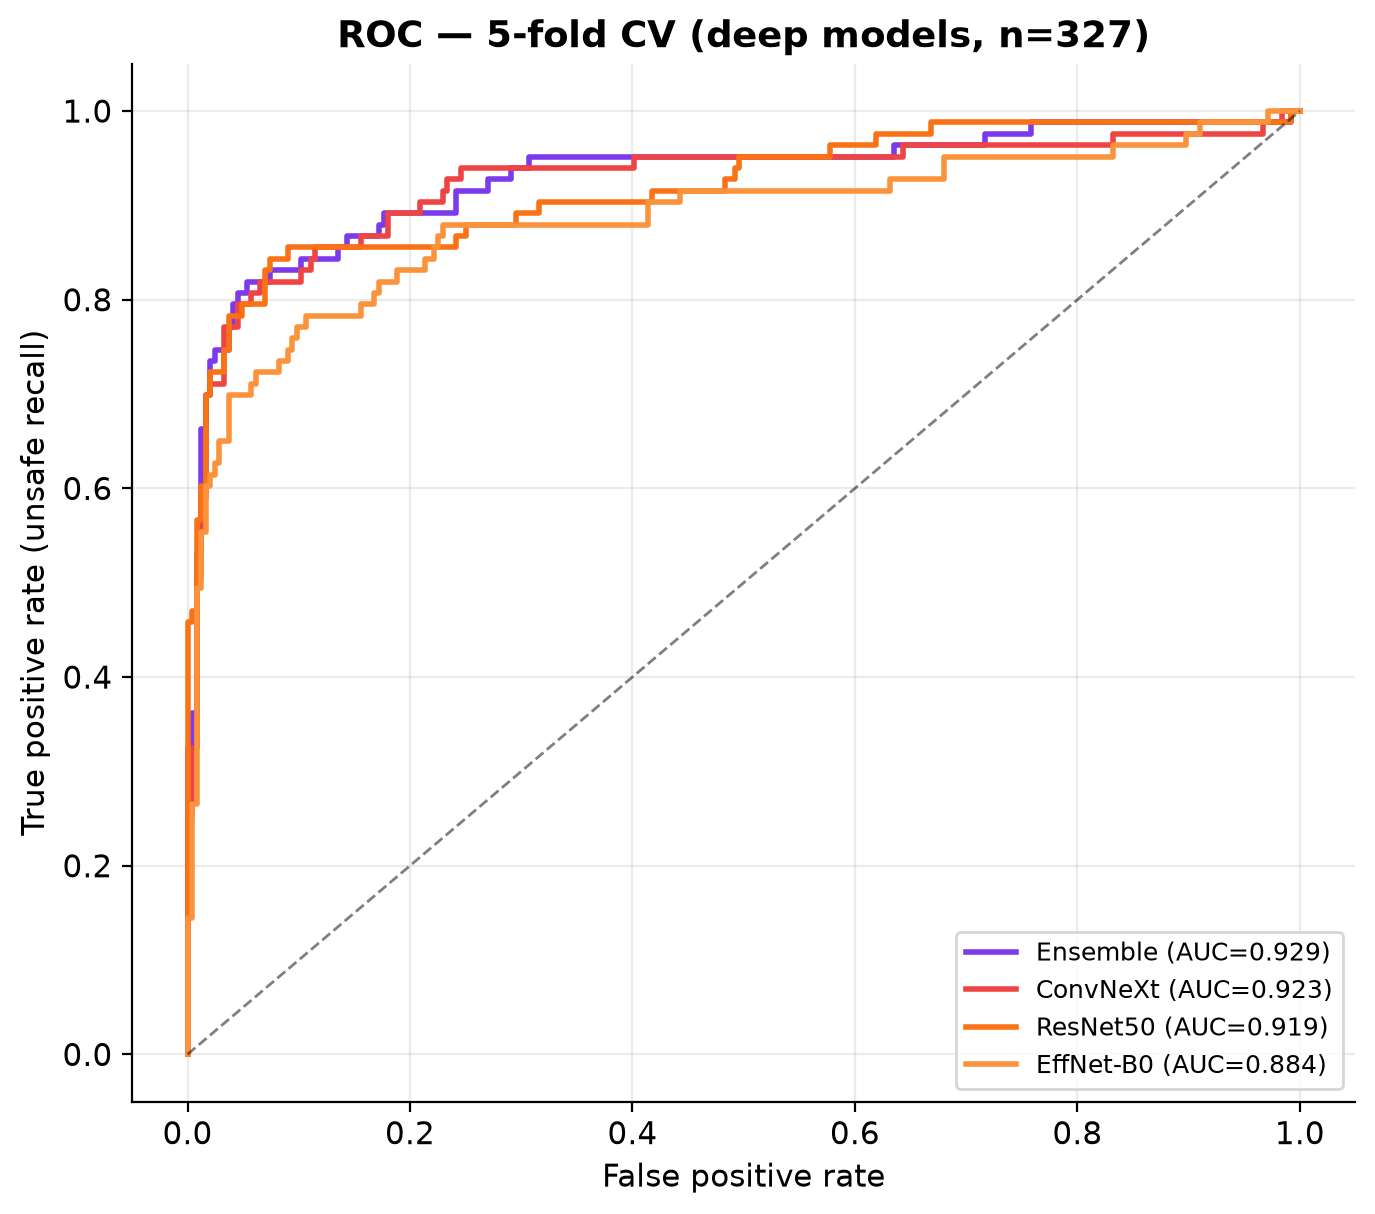
\includegraphics[width=\linewidth]{figures/fig8_roc_cv_deep.png}
    \caption{Cross-validated ROC curves for the deep models on the train+validation split.}
    \label{fig:paper_roc_cv_deep}
\end{figure}

\subsection{Error Analysis}
False negatives are the most safety-critical error type because they correspond to unsafe/risky hanging-travel cases predicted as safe/normal. The updated audit found that the 100\% recall threshold is dominated by a few difficult cases: one leguna image was identified as label noise, while other bus images contain very small or distant hanging passengers occupying only a small part of a cluttered frame. The deployed ensemble therefore provides selectable operating modes: balanced mode gives 91.7\% cross-validated accuracy and 80.7\% unsafe recall, high-recall mode gives 74.6\% accuracy and 95.2\% unsafe recall, and zero-miss mode reaches 100\% unsafe recall at only 26.0\% accuracy.

\section{Discussion}
\subsection{Interpretation of Results}
The updated results show that learned deep features outperform the classical HOG baselines at the balanced operating point. The ResNet50--ConvNeXt ensemble reached 91.7\% cross-validated accuracy, 80.7\% unsafe recall, and 0.929 AUC. ResNet50 alone produced the highest unsafe recall among balanced deep models at 84.3\%, while ConvNeXt-Tiny gave a similar AUC of 0.923.

Among classical models, SVM remains the strongest HOG baseline by AUC. HOG features encode local edge and gradient structure, which is useful for capturing vehicle outlines, doorway regions, and passenger posture cues. The RBF kernel further improves separability by modeling non-linear decision boundaries in this HOG feature space.

Gaussian Naive Bayes underperforms because its conditional-independence assumption is poorly matched to HOG descriptors. Neighboring gradient bins and block-normalized features are correlated by construction, so treating them as independent weakens the model's ability to distinguish visually similar safe/normal and unsafe/risky scenes.

The CNN trained from scratch reached the highest held-out test accuracy in the supplied table, but the 58-image test set is noisy and its unsafe recall was lower than the cross-validated high-recall operating point. The stronger cross-validated deep results indicate that transfer-learning backbones and ensembling provide the more reliable basis for deployment decisions.

\begin{figure}[!t]
    \centering
    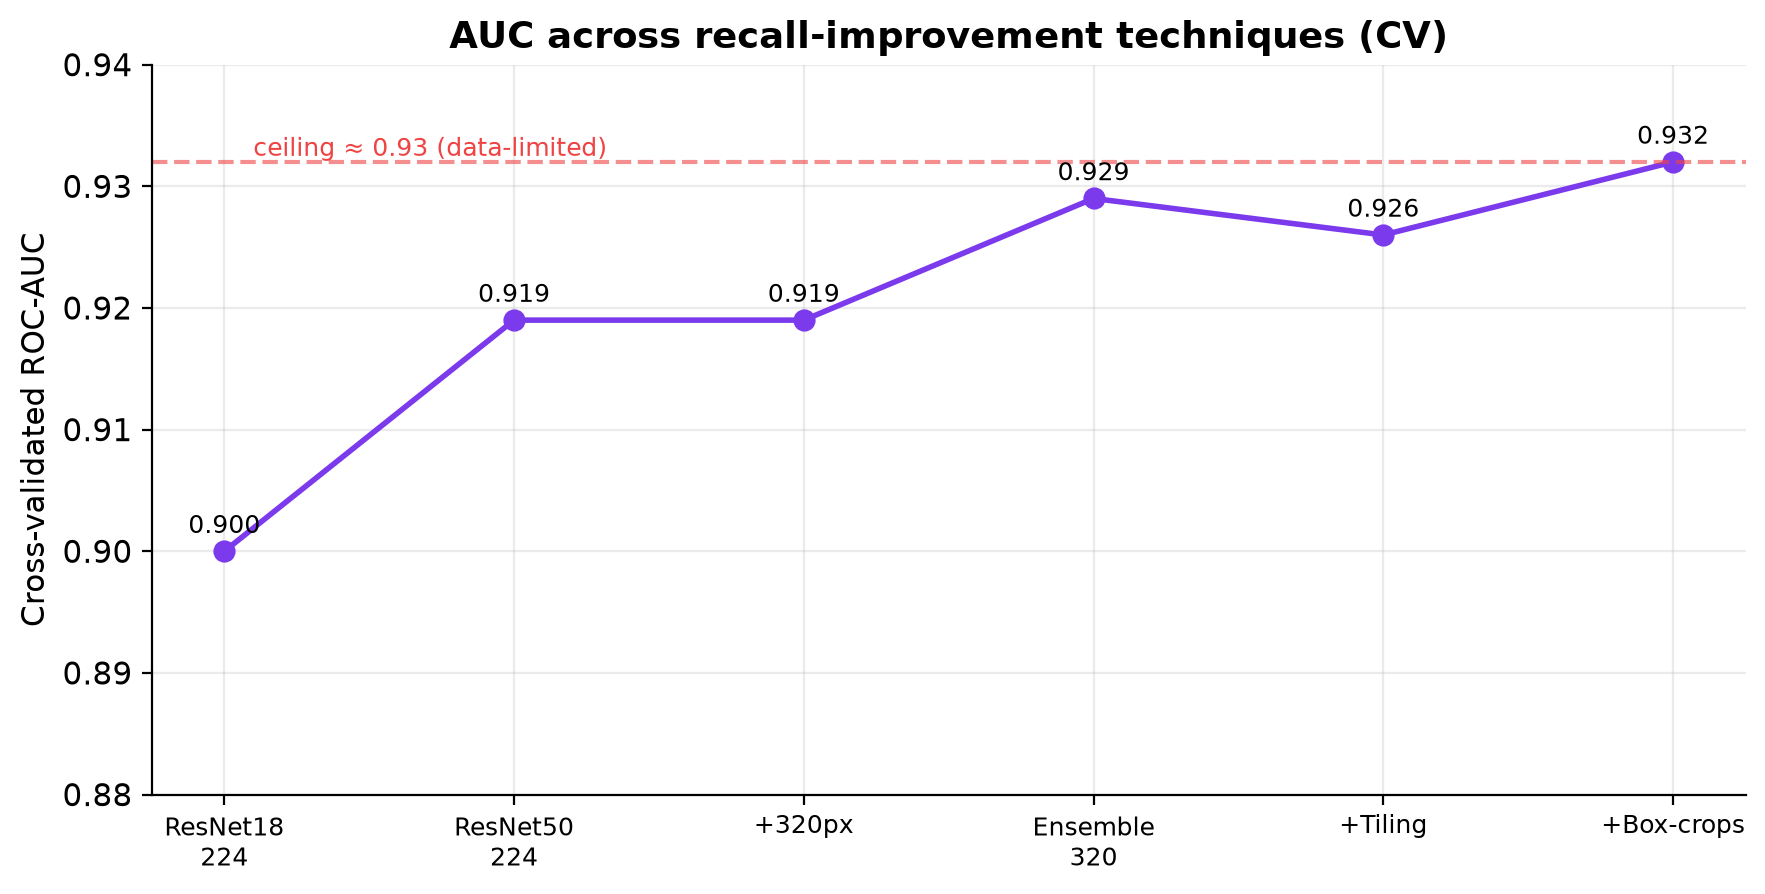
\includegraphics[width=\linewidth]{figures/fig7_technique_progression.png}
    \caption{Progression of recall-improvement techniques and the observed AUC ceiling in the paper assets.}
    \label{fig:paper_technique_progression}
\end{figure}

For this application, false negatives are more consequential than ordinary classification errors because they correspond to missed risky travel conditions. Precision and overall accuracy remain relevant for reducing false alarms, but a safety-oriented monitoring system should prioritize reducing missed unsafe cases while maintaining acceptable discrimination across normal and risky scenes.

\subsection{Limitations}
The main limitation of this study is the limited number of unique source images. The updated dataset contains 385 labeled images with 98 unsafe cases, which is still not enough to fully cover the diversity of vehicle layouts, camera viewpoints, passenger postures, weather, illumination, and traffic environments encountered in deployment.

The neural models also depend on training-time augmentation to increase effective sample diversity. Augmentation improves robustness to controlled transformations, but it does not replace additional real images containing natural occlusion, motion blur, dense crowding, and non-standard bus or leguna structures. These factors can make unsafe/risky positive cases difficult to distinguish from visually cluttered safe/normal scenes.

The current system is limited to image-level binary classification. It does not localize hanging passengers, estimate crowd density, track passengers across frames, or evaluate performance on large-scale real-time video streams. Roadside transport images may also include identifiable people, license plates, and location cues, so deployment would require anonymization and data-governance safeguards. The method should therefore be interpreted as a baseline for visual safety classification rather than an operational monitoring system.

\section{Conclusion and Future Work}
This paper presented a computer-vision and machine-learning pipeline for detecting unsafe hanging travel in Dhaka public transport. The task was formulated as binary image classification over safe/normal and unsafe/risky passenger conditions. A localized bus and leguna dataset was prepared through cleaning, annotation, preprocessing, and augmentation, with HOG features used for classical models and RGB inputs used for CNN-based classification.

The updated result set compares Logistic Regression, Gaussian Naive Bayes, SVM with an RBF kernel, a CNN trained from scratch, ResNet18, EfficientNet-B0, ResNet50, ConvNeXt-Tiny, and a ResNet50--ConvNeXt ensemble. The ensemble achieved the strongest balanced cross-validated result with 91.7\% accuracy, 80.7\% unsafe recall, and 0.929 AUC. For safety-oriented screening, the high-recall operating mode increased unsafe recall to 95.2\% at 74.6\% accuracy, while zero-miss mode reached 100\% unsafe recall with many false alarms.

Future work should focus on collecting a larger localized dataset, improving recall for unsafe hanging travel, evaluating the system on real-time video streams, and designing privacy-aware deployment procedures. Detection-based models such as YOLO \cite{redmon2016yolo} should also be tested to localize hanging passengers rather than only classify whole images. License-plate recognition may be integrated only as a future extension for vehicle identification after unsafe conditions are detected.

\begin{thebibliography}{99}

\bibitem{dilek2023cvits}
E. Dilek and M. Dener,
``Computer Vision Applications in Intelligent Transportation Systems: A Survey,''
\textit{Sensors}, vol. 23, no. 6, 2938, 2023.\\
Available: \url{https://www.mdpi.com/1424-8220/23/6/2938}

\bibitem{hsu2020passenger}
Y.-W. Hsu, T.-Y. Wang, and J.-W. Perng,
``Passenger flow counting in buses based on deep learning using surveillance video,''
\textit{Optik}, vol. 202, 163390, 2020.\\
Available: \url{https://www.sciencedirect.com/science/article/abs/pii/S0030402619315736}

\bibitem{hossain2018bus}
M. Hossain, M. A. Karim, and S. Rahman,
``Operational Hazards of Bus Transportation in Dhaka Metro City,''
\textit{Journal of Bangladesh Institute of Planners}, vol. 11, pp. 45-58, 2018.

\bibitem{crowding2023review}
S. Tirachini and D. A. Hensher,
``Crowding in Public Transport: A Review of Objective and Subjective Measures,''
\textit{Journal of Public Transportation}, vol. 24, 100058, 2022.\\
Available: \url{https://www.sciencedirect.com/science/article/pii/S1077291X22012486}

\bibitem{wastupranata2024abnormal}
L. M. Wastupranata and S. G. Kong,
``Deep Learning for Abnormal Human Behavior Detection in Surveillance Videos: A Survey,''
\textit{Electronics}, vol. 13, no. 13, 2579, 2024.\\
Available: \url{https://www.mdpi.com/2079-9292/13/13/2579}

\bibitem{redmon2016yolo}
J. Redmon, S. Divvala, R. Girshick, and A. Farhadi,
``You Only Look Once: Unified, Real-Time Object Detection,''
in \textit{IEEE Conference on Computer Vision and Pattern Recognition (CVPR)}, 2016, pp. 779-788.\\
Available: \url{https://arxiv.org/abs/1506.02640}

\bibitem{yolo2024boarding}
``A Study on Bus Passenger Boarding and Alighting Detection and Recognition Based on Video Images and the YOLO Algorithm,''
\textit{Sensors}, vol. 26, no. 5, 1418, 2026.\\
Available: \url{https://www.mdpi.com/1424-8220/26/5/1418}

\bibitem{anagnostopoulos2008license}
C. N. E. Anagnostopoulos, I. E. Anagnostopoulos, I. D. Psoroulas, V. Loumos, and E. Kayafas,
``License Plate Recognition From Still Images and Video Sequences: A Survey,''
\textit{IEEE Transactions on Intelligent Transportation Systems}, vol. 9, no. 3, pp. 377-391, 2008.\\
Available: \url{https://ieeexplore.ieee.org/document/4557614}

\bibitem{silva2018license}
S. M. Silva and C. R. Jung,
``License Plate Detection and Recognition in Unconstrained Scenarios,''
in \textit{European Conference on Computer Vision (ECCV)}, 2018, pp. 580-596.\\
Available: \url{https://link.springer.com/chapter/10.1007/978-3-030-01258-8_35}

\bibitem{du2013automatic}
S. Du, M. Ibrahim, M. Shehata, and W. Badawy,
``Automatic License Plate Recognition (ALPR): A State-of-the-Art Review,''
\textit{IEEE Transactions on Circuits and Systems for Video Technology}, vol. 23, no. 2, pp. 311-325, 2013.\\
Available: \url{https://doi.org/10.1109/TCSVT.2012.2203741}

\bibitem{afrin2023bengali}
N. Afrin, M. M. Hasan, M. F. E. Safin, K. R. Amin, M. Z. Haque, F. Ahmed, and M. T. R. Shawon,
``Bengali License Plate Recognition: Unveiling Clarity with CNN and GFP-GAN,''
in \textit{26th International Conference on Computer and Information Technology (ICCIT)}, Cox's Bazar, Bangladesh, 2023, pp. 1-6.\\
Available: \url{https://arxiv.org/abs/2312.10701}

\bibitem{shorten2019augmentation}
C. Shorten and T. M. Khoshgoftaar,
``A survey on Image Data Augmentation for Deep Learning,''
\textit{Journal of Big Data}, vol. 6, art. 60, 2019.\\
Available: \url{https://link.springer.com/article/10.1186/s40537-019-0197-0}

\bibitem{dalal2005hog}
N. Dalal and B. Triggs,
``Histograms of Oriented Gradients for Human Detection,''
in \textit{IEEE Conference on Computer Vision and Pattern Recognition (CVPR)}, 2005, pp. 886-893.\\
Available: \url{https://lear.inrialpes.fr/people/triggs/pubs/Dalal-cvpr05.pdf}

\bibitem{vanderwalt2014skimage}
S. van der Walt, J. L. Sch\"onberger, J. Nunez-Iglesias, F. Boulogne, J. D. Warner, N. Yager, E. Gouillart, and T. Yu,
``scikit-image: image processing in Python,''
\textit{PeerJ}, vol. 2, e453, 2014.\\
Available: \url{https://peerj.com/articles/453/}

\bibitem{cortes1995svm}
C. Cortes and V. Vapnik,
``Support-Vector Networks,''
\textit{Machine Learning}, vol. 20, no. 3, pp. 273-297, 1995.\\
Available: \url{https://link.springer.com/article/10.1007/BF00994018}

\bibitem{krizhevsky2012alexnet}
A. Krizhevsky, I. Sutskever, and G. E. Hinton,
``ImageNet Classification with Deep Convolutional Neural Networks,''
in \textit{Advances in Neural Information Processing Systems (NeurIPS)}, vol. 25, 2012, pp. 1097-1105.\\
Available: \url{https://papers.nips.cc/paper/4824-imagenet-classification-with-deep-convolutional-neural-networks}

\bibitem{he2016resnet}
K. He, X. Zhang, S. Ren, and J. Sun,
``Deep Residual Learning for Image Recognition,''
in \textit{IEEE Conference on Computer Vision and Pattern Recognition (CVPR)}, 2016, pp. 770-778.\\
Available: \url{https://arxiv.org/abs/1512.03385}

\bibitem{tan2019efficientnet}
M. Tan and Q. V. Le,
``EfficientNet: Rethinking Model Scaling for Convolutional Neural Networks,''
in \textit{International Conference on Machine Learning (ICML)}, 2019, pp. 6105-6114.\\
Available: \url{https://arxiv.org/abs/1905.11946}

\bibitem{liu2022convnext}
Z. Liu, H. Mao, C.-Y. Wu, C. Feichtenhofer, T. Darrell, and S. Xie,
``A ConvNet for the 2020s,''
in \textit{IEEE Conference on Computer Vision and Pattern Recognition (CVPR)}, 2022, pp. 11976-11986.\\
Available: \url{https://arxiv.org/abs/2201.03545}

\bibitem{ioffe2015batchnorm}
S. Ioffe and C. Szegedy,
``Batch Normalization: Accelerating Deep Network Training by Reducing Internal Covariate Shift,''
in \textit{International Conference on Machine Learning (ICML)}, 2015, pp. 448-456.\\
Available: \url{https://arxiv.org/abs/1502.03167}

\bibitem{srivastava2014dropout}
N. Srivastava, G. Hinton, A. Krizhevsky, I. Sutskever, and R. Salakhutdinov,
``Dropout: A Simple Way to Prevent Neural Networks from Overfitting,''
\textit{Journal of Machine Learning Research}, vol. 15, pp. 1929-1958, 2014.\\
Available: \url{https://jmlr.org/papers/v15/srivastava14a.html}

\bibitem{pedregosa2011sklearn}
F. Pedregosa et al.,
``Scikit-learn: Machine Learning in Python,''
\textit{Journal of Machine Learning Research}, vol. 12, pp. 2825-2830, 2011.\\
Available: \url{https://jmlr.org/papers/v12/pedregosa11a.html}

\bibitem{paszke2019pytorch}
A. Paszke et al.,
``PyTorch: An Imperative Style, High-Performance Deep Learning Library,''
in \textit{Advances in Neural Information Processing Systems (NeurIPS)}, vol. 32, 2019, pp. 8024-8035.\\
Available: \url{https://papers.nips.cc/paper/9015-pytorch-an-imperative-style-high-performance-deep-learning-library}

\bibitem{kingma2015adam}
D. P. Kingma and J. Ba,
``Adam: A Method for Stochastic Optimization,''
in \textit{International Conference on Learning Representations (ICLR)}, 2015.\\
Available: \url{https://arxiv.org/abs/1412.6980}

\end{thebibliography}

\end{document}
